% CHAPITRE 3 — Réalisation de la plateforme PlainteCam

\chapter{Réalisation de la plateforme PlainteCam}
\label{ch:realisation}
\label{ch:bilan}

Le chapitre précédent a fixé ce que la plateforme doit faire et comment elle s'organise. Celui-ci rend compte de sa réalisation effective, puis de ce qu'elle vaut une fois construite.

Il s'ouvre sur le choix des outils et des technologies retenus pour porter la conception, puis sur l'architecture d'implémentation, qui montre comment ces technologies s'assemblent et communiquent. Il détaille ensuite la mise en œuvre de la solution, du parcours de dépôt jusqu'aux tests de recette. Il analyse alors les résultats obtenus en précisant la portée exacte des mesures, expose les apports pour l'organisation, formule les préconisations de pérennisation et dresse le bilan critique de la mission. Il se referme sur la présentation des interfaces effectivement livrées, qui donne à voir l'application réalisée.

\section{Choix des outils et technologies}

Réaliser la conception arrêtée au chapitre~\ref{ch:conception} supposait d'abord de choisir les technologies qui la porteraient. Ce choix a été guidé par trois contraintes issues du diagnostic : un public non technicien, une intégration d'intelligence artificielle sans friction, et un coût d'exploitation compatible avec les moyens d'une administration.

\subsection{Frontend : React.js}

Pour le frontend, React.js a été sélectionné après évaluation comparative des technologies d'interface utilisateur web les plus répandues. Vue.js offre une courbe d'apprentissage plus douce mais un écosystème plus restreint, tandis qu'Angular impose une structure complète dont la rigidité ne se justifiait pas à l'échelle du projet.

React a été retenu parce que ses composants permettent aux quatre espaces de partager les mêmes briques d'interface sans duplication, et parce que sa gestion d'état convient au formulaire de dépôt en cinq étapes, dont la saisie doit survivre à la navigation entre écrans.

\begin{figure}[H]
    \centering
    
\includegraphics[width=0.22\textwidth]{images/react.png}
    \caption{React.js, bibliothèque frontend}
    \label{fig:react}
\end{figure}

\subsection{Backend : Flask}

\textbf{Flask} a été retenu pour l'exposition des API et l'orchestration de la logique métier côté serveur. Ce micro-framework Python suit la spécification \textbf{WSGI} et laisse au développeur le choix de ses composants plutôt que d'imposer une pile complète, à la différence de Django dont les conventions nombreuses auraient alourdi un périmètre maîtrisé.

Flask a été retenu d'abord pour la \textbf{continuité de langage avec l'intelligence artificielle} : le client Python de Groq s'intègre au backend sans passerelle ni service intermédiaire, et c'est le critère qui a tranché. Il l'a été ensuite parce qu'un périmètre fonctionnel maîtrisé permet de choisir explicitement chaque brique plutôt que d'en hériter d'une pile imposée, avec SQLAlchemy pour la persistance et Flask-JWT-Extended pour l'authentification, pour une empreinte et un coût d'exploitation réduits derrière un serveur WSGI de production.

% La figure s'affiche automatiquement dès que images/flask.png existe.
\IfFileExists{images/flask.png}{%
\begin{figure}[H]
    \centering
    
\includegraphics[width=0.28\textwidth]{images/flask.png}
    \caption{Flask, micro-framework backend Python}
    \label{fig:flask}
\end{figure}
}{}

\subsection{Persistance : PostgreSQL et Supabase Storage}

Le \textbf{SGBD PostgreSQL} assure la persistance des données structurées. Son typage fort, ses types énumérés natifs pour les statuts, les priorités et les natures d'infraction, ainsi que son moteur transactionnel garantissent la cohérence des dossiers tout au long de l'enquête.

Les \textbf{pièces jointes} sont en revanche confiées à \textbf{Supabase Storage}, la base ne conservant que leurs métadonnées et le chemin de l'objet. Le dépôt est un \textbf{bucket privé} réservé aux utilisateurs authentifiés : aucune pièce n'est accessible par une URL publique, ce qui serait inacceptable pour un certificat médical ou l'identité d'un mis en cause. Ce choix répond directement au besoin de confidentialité (BNF1).

\subsection{Intelligence artificielle : Llama 3.1 servi par Groq}

La rédaction assistée des procès-verbaux s'appuie sur le modèle \textbf{Llama 3.1} de Meta, exploité via la plateforme d'inférence \textbf{Groq}, à ne pas confondre avec \textit{Grok}, le modèle de la société xAI. Son \textbf{palier gratuit} couvre les besoins du projet, son inférence rapide rend la proposition quasi instantanée, les poids ouverts de Llama autorisent un réhébergement ultérieur sur infrastructure maîtrisée, et l'appel reste exclusivement côté serveur : la clé d'API n'est jamais exposée au navigateur.

Le procès-verbal produit reste une \textbf{proposition}. Il est présenté à l'enquêteur dans un éditeur, qui le corrige et le valide avant signature. L'intelligence artificielle assiste la rédaction, elle ne se substitue pas à l'officier de police judiciaire, seul habilité à dresser le procès-verbal au sens du Code de procédure pénale~\cite{cameroun-cpp}. C'est la traduction technique du besoin de valeur probante (BNF3).

\begin{figure}[H]
    \centering
    
\includegraphics[width=0.34\textwidth]{images/grok_ai.png}
    \caption{Intelligence artificielle générative intégrée à PlainteCam}
    \label{fig:ia}
\end{figure}

\subsection{Environnement de développement}

Le développement s'est effectué sous \textbf{Windows 10}, avec \textbf{Visual Studio Code} pour l'édition du frontend React et du backend Python. Le versionnement est assuré par \textbf{Git} et \textbf{GitHub}. \textbf{Docker} conteneurise l'API et le SGBD : le backend Python et PostgreSQL s'exécutent ainsi dans un environnement Linux identique à celui visé en production, ce qui neutralise les écarts entre le poste de développement Windows et le serveur cible, qu'il s'agisse des chemins de fichiers, des fins de ligne ou des dépendances système. Enfin, \textbf{Postman} a servi à la recette des endpoints REST avant leur intégration au frontend.

\section{Architecture d'implémentation}

Ces technologies étant arrêtées, il reste à montrer comment elles s'assemblent et par quels protocoles elles communiquent.

La figure~\ref{fig:archi_implementation} traduit la conception en technologies. La plateforme suit une architecture \textbf{trois-tiers découplée} : le frontend React.js communique exclusivement avec le backend Flask via des API REST sécurisées par jeton. Le backend orchestre la logique métier, la persistance des données et les appels au service d'intelligence artificielle générative.

\begin{figure}[H]
    \centering
    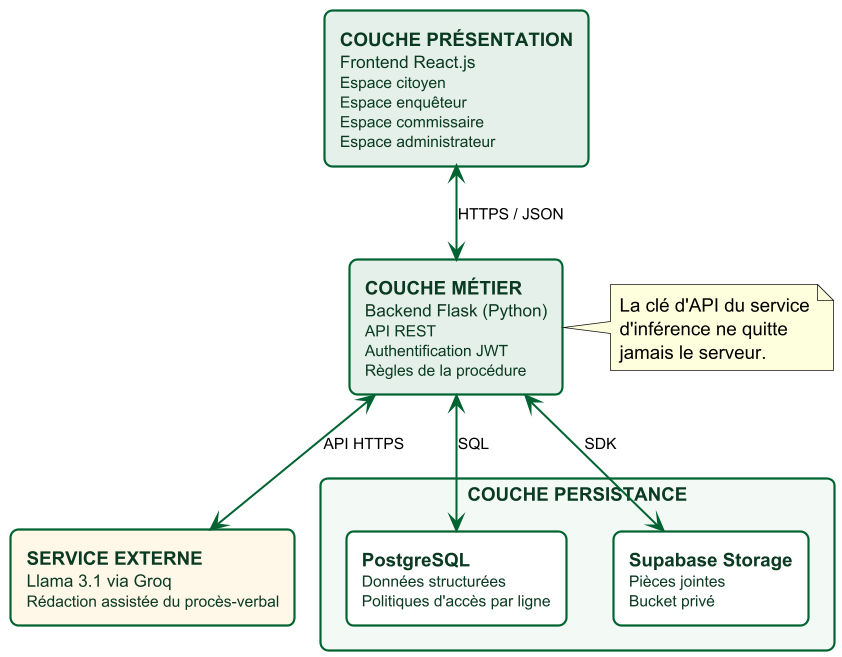
\includegraphics[width=0.78\textwidth]{diagrammes/architecture.png}
    \caption{Architecture d'implémentation : technologies et communications}
    \label{fig:archi_implementation}
\end{figure}

Les échanges portent chacun leur protocole : \textbf{HTTPS} et \textbf{JSON} entre la présentation et le métier, \textbf{SQL} vers PostgreSQL, un \textbf{SDK} vers le dépôt d'objets, et un appel \textbf{HTTPS} vers le service d'inférence. Cette dernière liaison n'existe qu'entre le backend et Groq, jamais depuis le navigateur. C'est ce qui garantit que la clé d'API ne quitte pas le serveur.

\section{Mise en œuvre de la solution}

Cette section décrit comment les besoins fonctionnels et non fonctionnels énoncés au chapitre précédent ont été effectivement implémentés, en partant du parcours le plus visible pour l'utilisateur pour aller vers les mécanismes qui le soutiennent.

\subsection{Parcours de dépôt du plaignant}

Le dépôt de plainte est implémenté comme un \textbf{formulaire séquentiel} en cinq écrans enchaînés :

\begin{enumerate}
    \item \textbf{Nature de l'infraction.} Choix parmi les natures gérées : vol simple, vol avec violence, agression physique, escroquerie, harcèlement, dégradation de biens, accident de la route, autre. Le \textbf{cumul est possible}, une même affaire pouvant relever de plusieurs qualifications, par exemple une escroquerie doublée d'un abus de confiance. Suit la cascade géographique Région, Département, Arrondissement, Quartier, dont le \textbf{commissariat compétent} est déduit automatiquement.
    \item \textbf{Déclaration des faits.} Récit libre du plaignant, avec dictée vocale optionnelle s'appuyant sur la Web Speech API du navigateur.
    \item \textbf{Identité du mis en cause.} Renseignée lorsqu'elle est connue, facultative dans le cas contraire.
    \item \textbf{Questions complémentaires.} Un jeu de questions propre à la nature de l'infraction est proposé. Celles dont la réponse figure déjà dans le récit des faits sont automatiquement écartées, afin de ne pas faire répéter le plaignant.
    \item \textbf{Aperçu et confirmation.} Récapitulatif de la déclaration, signature puis dépôt définitif, avec délivrance d'un \textbf{récépissé} portant le numéro de dossier.
\end{enumerate}

\paragraph{Analyse en direct de la déclaration.} Pendant que le plaignant rédige son récit, un bloc d'analyse affiche en continu un \textbf{taux de complétude} : la part des éléments attendus pour la nature d'infraction déclarée, à savoir l'objet concerné, le moment des faits, la description du suspect, les témoins et le justificatif, effectivement repérés dans le texte. Chaque élément apparaît sous forme d'étiquette, verte s'il est présent, rouge s'il manque, et une jauge situe le niveau atteint : rouge en dessous de 50~\%, orange de 50 à 80~\%, vert au-delà.

Ce pourcentage n'a qu'une seule fonction : \textbf{montrer au plaignant ce qui manque encore à sa déclaration}, afin qu'il le complète de lui-même avant de poursuivre. Il ne mesure ni la gravité des faits, ni l'avancement du dossier. Les éléments restés non détectés deviennent précisément les questions posées à l'étape 4, ce qui évite d'interroger le plaignant sur ce qu'il a déjà écrit.

\paragraph{Choix retenu pour la compétence territoriale.} L'audit a établi que le commissariat compétent peut être celui du lieu des faits \textbf{ou} celui du secteur de résidence du mis en cause. La plateforme retient le \textbf{lieu des faits}, seul critère systématiquement connu du plaignant au moment du dépôt, l'identité du mis en cause et a fortiori son adresse étant fréquemment ignorées. Ce choix ne ferme aucune option : le commissariat destinataire conserve la faculté de se dessaisir au profit d'une autre unité, le transfert étant alors inscrit au journal d'audit.

\subsection{Du dépôt à la clôture : le cycle de vie du dossier}

Une fois la plainte déposée, le dossier est rattaché au commissariat compétent et apparaît dans le tableau de bord du \textbf{commissaire}. Celui-ci procède à la \textbf{cotation} : il désigne l'\textbf{enquêteur} chargé de l'affaire et fixe la priorité du dossier.

L'enquêteur conduit ensuite l'instruction. Il convoque le plaignant et le mis en cause, tient les \textbf{auditions} et dresse les \textbf{procès-verbaux} correspondants. Chaque changement d'état est inscrit au journal d'audit. Le statut du dossier suit un cycle contraint par un type énuméré : \textit{Reçu}, \textit{Audition}, \textit{En instruction}, \textit{Décision}, \textit{Transmis}, \textit{Clôturé}. Le plaignant suit cette progression depuis son espace, sans avoir à se déplacer ni à téléphoner.

L'\textbf{avancement du dossier} est calculé comme la part de la procédure réellement accomplie : les étapes franchies, plus la fraction des actes déjà réalisés au sein de l'étape en cours. Un dossier transmis au parquet ou clôturé est à 100~\%. Cette valeur ne se saisit jamais à la main, de sorte qu'un dossier ne peut pas être déclaré avancé sans que les actes correspondants figurent effectivement au dossier. L'enquêteur la retrouve détaillée dans son \textbf{étapier}, une frise qui énumère pour chaque étape les actes requis et barre ceux qui sont accomplis ; le commissaire en suit la moyenne sur son tableau de bord.

Ces deux pourcentages ne mesurent donc pas la même chose et ne s'adressent pas aux mêmes personnes. La \textbf{complétude} qualifie la \textit{déclaration} et regarde le citoyen pendant qu'il rédige ; l'\textbf{avancement} qualifie la \textit{procédure} et regarde le commissaire qui supervise. Les confondre conduirait à présenter comme avancé un dossier simplement bien raconté, alors que rien n'y aurait encore été fait.

\subsection{Modèle de données}

Le schéma relationnel compte huit entités, dont le rôle est décrit ci-dessous.

\begin{itemize}
    \item \textbf{Commissariat.} Référentiel des commissariats et de leur ressort territorial, en lecture publique puisqu'il sert la cascade géographique du dépôt.
    \item \textbf{Profil.} Citoyens et personnels, porteurs du rôle applicatif qui détermine leurs droits.
    \item \textbf{Plainte.} Dossiers déposés et leur cycle de vie complet. Une plainte porte une ou plusieurs qualifications et un ou plusieurs préjudices, et n'est accessible qu'au plaignant et au commissariat saisi.
    \item \textbf{Pièce jointe.} Métadonnées des documents et photos, le fichier lui-même résidant dans le dépôt d'objets. L'accès est restreint au dossier de rattachement.
    \item \textbf{Procès-verbal.} Procès-verbaux d'audition proposés par l'intelligence artificielle puis validés par l'enquêteur, accessibles à ce dernier seul.
    \item \textbf{Convocation.} Convocations émises et suites données, visibles du commissariat émetteur.
    \item \textbf{Historique.} Journal d'audit de toutes les transitions de statut, en lecture seule y compris pour les administrateurs.
    \item \textbf{Notification.} Messages adressés au plaignant et aux personnels, visibles de leur seul destinataire.
\end{itemize}

\subsection{Sécurité et contrôle d'accès}

L'authentification repose sur des jetons \textbf{JWT}~\cite{jwt-rfc} signés côté serveur. Le citoyen s'identifie par adresse électronique et code à usage unique ; les personnels par matricule et mot de passe. Chaque requête est ensuite autorisée selon le rôle porté par le jeton : un plaignant n'accède qu'à ses propres dossiers, un enquêteur à ceux qui lui ont été cotés, un commissaire à l'ensemble des dossiers de son commissariat. Ce cloisonnement est doublé au niveau du SGBD par des politiques d'accès par ligne, de sorte qu'une requête mal formée ne puisse pas contourner la règle métier. C'est ce double verrou, applicatif et base de données, qui satisfait le besoin de confidentialité (BNF1).

\subsection{Tests effectués}

La recette a été conduite manuellement sur un jeu de dossiers de test couvrant les huit natures d'infraction gérées. Elle a porté sur quatre familles de scénarios, dont le détail figure en annexe~C.

Les \textbf{tests fonctionnels} ont vérifié le dépôt complet d'une plainte sur les cinq étapes du parcours, la détermination du commissariat compétent par cascade géographique, et la cotation d'un dossier à un enquêteur avec fixation de la priorité. Les trois se sont révélés conformes.

Le \textbf{test d'intelligence artificielle} a porté sur la rédaction d'un procès-verbal à partir de la déclaration du plaignant. Le résultat est conforme, sous la réserve constante que la relecture de l'enquêteur reste requise.

Les \textbf{tests de sécurité} ont cherché à mettre le cloisonnement en défaut. La consultation d'un dossier tiers par un citoyen non plaignant a été refusée, de même que l'appel d'un point d'accès sans jeton valide, rejeté par un code HTTP 401. Dans les deux cas, c'est le refus qui constitue le succès du test.

Les \textbf{tests documentaires et de qualité} ont contrôlé la génération des PDF du récépissé et du procès-verbal ainsi que la validité du QR code, tous conformes. La fidélité de la transcription vocale, en revanche, n'est que partiellement satisfaisante et impose une relecture.

Deux limites sont assumées à ce stade. La dictée vocale fonctionne sur l'ensemble des navigateurs testés, mais la \textbf{fidélité de la transcription reste imparfaite} : le texte obtenu ne restitue pas toujours exactement les propos du plaignant, en particulier sur les noms propres, les toponymes et les tournures propres au français parlé localement. Une relecture à l'écran est donc indispensable avant de passer à l'étape suivante, et la dictée est présentée comme une aide à la saisie plutôt que comme un mode de déclaration autonome. Par ailleurs, aucun test de charge n'a été mené faute d'environnement de production représentatif. Ces deux points figurent dans les préconisations formulées plus loin.

\section{Analyse des résultats}

La plateforme étant réalisée et testée, reste à établir ce qu'elle change effectivement, et avec quel degré de certitude.

\subsection{Méthode de mesure}

Les résultats présentés ci-dessous ont été relevés en \textbf{recette}, sur un jeu de dossiers de test couvrant les huit natures d'infraction gérées, et non en exploitation réelle. Les valeurs « avant » décrivent la procédure telle que l'audit l'a documentée ; les valeurs « après » ont été relevées sur la plateforme.

Une précision de méthode s'impose ici. Le mémoire \textbf{n'avance aucun chiffre sur la durée de cotation d'un dossier ni sur celle de traitement d'une affaire}. Ces durées relèvent de la connaissance interne du commissariat, varient fortement selon l'affluence, la nature des faits et la disponibilité des enquêteurs, et aucune source ne permettait de les établir : c'est précisément l'absence de traçabilité qui les rend inconnaissables. Les avancer aurait été une extrapolation. Le tableau ne compare donc que ce qui a pu être constaté de part et d'autre, et signale explicitement, en dernière ligne, ce que la plateforme rend désormais \textbf{mesurable} sans prétendre en connaître la valeur.

\begin{table}[H]
    \centering
    \begin{tabularx}{\textwidth}{|>{\raggedright\arraybackslash}X|>{\raggedright\arraybackslash}p{2.4cm}|>{\raggedright\arraybackslash}p{2.9cm}|>{\raggedright\arraybackslash}p{2.2cm}|}
        \hline
        \textbf{Indicateur} & \textbf{Avant} & \textbf{Après} & \textbf{Nature} \\
        \hline
        Déplacement pour déposer plainte & Obligatoire & Supprimé & Mesuré \\
        \hline
        Saisie de la déclaration par le plaignant & Au guichet, tributaire de l'affluence & $<$ 8 min en ligne & Mesuré \\
        \hline
        Détermination du commissariat compétent & Oralement au guichet & Automatique, par le lieu des faits & Mesuré \\
        \hline
        Mise en forme d'un procès-verbal & Manuscrite, sur template papier & Proposition structurée en $<$ 2 min, à réviser & Mesuré \\
        \hline
        Complétude de la déclaration & Variable selon l'aisance du plaignant & Questions ciblées et score de complétude & Mesuré \\
        \hline
        Traçabilité des actes de procédure & Registre papier & 100\% horodatée & Mesuré \\
        \hline
        Suivi du dossier par le plaignant & Déplacement nécessaire & Disponible en ligne & Mesuré \\
        \hline
        Remise de la convocation au mis en cause & À la charge du plaignant & Notification par la plateforme & Mesuré \\
        \hline
        Délai entre dépôt et cotation & \textbf{Non mesurable} & Horodaté, donc mesurable & Nouvelle capacité \\
        \hline
        Taux d'erreur dans les procès-verbaux & Non mesuré & Non mesuré & À instrumenter \\
        \hline
    \end{tabularx}
    \caption{Comparaison des indicateurs avant et après PlainteCam}
    \label{tab:resultats}
\end{table}

\subsection{Portée et limites des mesures}

Trois réserves doivent accompagner la lecture de ce tableau. D'abord, les durées « après » sont celles d'un utilisateur accompagné en recette, non celles d'un citoyen livré à lui-même ; l'écart réel sera plus élevé. Ensuite, la proposition de procès-verbal produite en moins de deux minutes doit encore être relue et corrigée par l'enquêteur : le gain porte sur la mise en forme et la structuration, non sur l'appréciation juridique des faits. Enfin, aucun test de charge n'a été mené, faute d'environnement de production représentatif ; les temps de réponse observés ne préjugent pas du comportement de la plateforme en usage réel.

Il faut ajouter que la plateforme n'agit pas sur ce que l'audit a identifié comme la principale source de contentieux : le refus, par le mis en cause, de signer un procès-verbal dont il conteste la fidélité. La plateforme en conserve la trace horodatée, mais la situation reste entière. Annoncer une réduction des délais de traitement serait donc doublement infondé, faute de mesure initiale, et parce que ce facteur de blocage échappe à l'outil.

\section{Apports pour l'organisation}

Les mesures qui précèdent se traduisent, pour le commissariat, par quatre gains de nature différente.

\textbf{Gain de temps :} La suppression du déplacement et le rattachement automatique au commissariat compétent retirent de la chaîne les étapes de circulation physique qui précédaient toute action d'enquête. La rédaction assistée libère par ailleurs l'enquêteur d'une part importante du travail de mise en forme. L'ampleur de ce gain reste à établir en exploitation : elle dépend de la charge du service, que seul le commissariat connaît.

\textbf{Gain de qualité :} Le questionnaire complémentaire garantit qu'aucune information déterminante pour la nature d'infraction déclarée n'est omise au dépôt, là où la retranscription orale dépendait de la disponibilité et de l'expérience de l'agent de permanence.

\textbf{Gain de visibilité :} Le commissaire dispose pour la première fois d'indicateurs consolidés, qu'il s'agisse des volumes, des répartitions ou de la charge par enquêteur, pour piloter l'activité de son unité.

\textbf{Gain de traçabilité :} Chaque acte étant horodaté et attribué, la reconstitution d'une procédure devient immédiate, ce qui sert autant l'audit interne que la réponse aux demandes de l'autorité judiciaire.

\section{Préconisations}

Pour pérenniser et faire évoluer PlainteCam après la fin du stage, les préconisations suivantes sont formulées :

\begin{itemize}
    \item \textbf{Instrumenter la plateforme avant le déploiement :} enregistrer les durées réelles de dépôt, de cotation et de clôture afin de disposer d'indicateurs mesurés en exploitation, et non plus estimés en recette. C'est la condition pour objectiver le gain auprès de la hiérarchie.
    \item \textbf{Conduire un test de charge} représentatif du volume d'un commissariat urbain avant la mise en service.
    \item \textbf{Former les personnels}, en insistant sur la révision des procès-verbaux proposés par l'intelligence artificielle : le risque principal est la validation sans relecture d'un texte plausible mais inexact.
    \item \textbf{Améliorer la fidélité de la transcription vocale}, aujourd'hui inégale sur les noms propres et les toponymes. Une transcription côté serveur, entraînée ou adaptée au français parlé au Cameroun, corrigerait ce défaut. Tant qu'il subsiste, la relecture du texte dicté doit rester obligatoire avant validation.
    \item \textbf{Vérifier les quotas du service d'inférence avant la mise en service :} le projet fonctionne sur le palier gratuit de Groq, dont les limites de requêtes conviennent à un pilote, mais pas nécessairement au volume d'un commissariat urbain. Deux issues sont possibles selon l'arbitrage budgétaire, souscrire une offre payante ou réhéberger Llama sur un serveur de l'institution, ce que ses poids ouverts autorisent.
    \item \textbf{Désigner un référent technique interne} chargé des mises à jour, de la correction des anomalies et de l'évolution de la plateforme.
    \item \textbf{Déployer progressivement}, en commençant par un commissariat pilote, avant extension au reste du ressort.
\end{itemize}

\section{Bilan critique de la mission}

Au-delà des résultats mesurés, la conduite du projet appelle un retour réflexif sur ce qui a facilité le travail et ce qui l'a entravé.

\subsection{Ce qui a fonctionné}

Quatre choix se sont révélés payants au fil de la mission.

\begin{itemize}
    \item La méthodologie Agile a permis de livrer des fonctionnalités utilisables dès le deuxième sprint, facilitant les retours précoces des parties prenantes.
    \item Le choix de Python pour le backend a supprimé toute friction dans l'intégration de l'intelligence artificielle générative, qui s'est faite plus vite que prévu.
    \item L'architecture découplée entre frontend et backend a permis un développement parallèle efficace des deux couches.
    \item Le questionnaire complémentaire, conçu avec les personnels du commissariat, s'est révélé mieux accepté que la génération automatique seule, parce qu'il laisse la main au plaignant.
\end{itemize}

\subsection{Ce qui a posé des défis}

Quatre difficultés ont en revanche pesé sur le déroulement du projet.

\begin{itemize}
    \item La modélisation géographique en cascade a demandé plus de temps que prévu, les données de référence des quartiers étant incomplètes et hétérogènes.
    \item La gestion des droits d'accès par rôle a nécessité plusieurs itérations avant d'atteindre un niveau de cloisonnement satisfaisant entre plaignant, enquêteur et commissaire.
    \item La question de la valeur probante du dossier numérique a été sous-estimée au départ : elle relève autant du juridique que de la technique et aurait mérité d'être instruite dès la conception.
    \item La conduite du changement auprès des personnels a demandé un effort de formation et de communication plus important que planifié.
\end{itemize}

\subsection{Enseignements tirés}

Cette mission a confirmé l'importance d'impliquer les utilisateurs finaux dès la phase de conception pour éviter les allers-retours coûteux en fin de projet. Elle a également montré qu'un projet de dématérialisation dans un contexte régalien ne se réduit pas à un problème technique : les dimensions juridiques et organisationnelles conditionnent l'adoption autant que la qualité du logiciel. Enfin, elle a mis en évidence la nécessité d'instrumenter une plateforme dès sa conception, faute de quoi la démonstration de sa valeur repose sur des estimations plutôt que sur des mesures.

\section{Résultats : interfaces de la plateforme}

Cette dernière section donne à voir le produit fini. Chaque interface y est rapportée au besoin fonctionnel qu'elle satisfait.

\subsection{Tableau de bord du commissaire}

\begin{figure}[H]
    \centering
    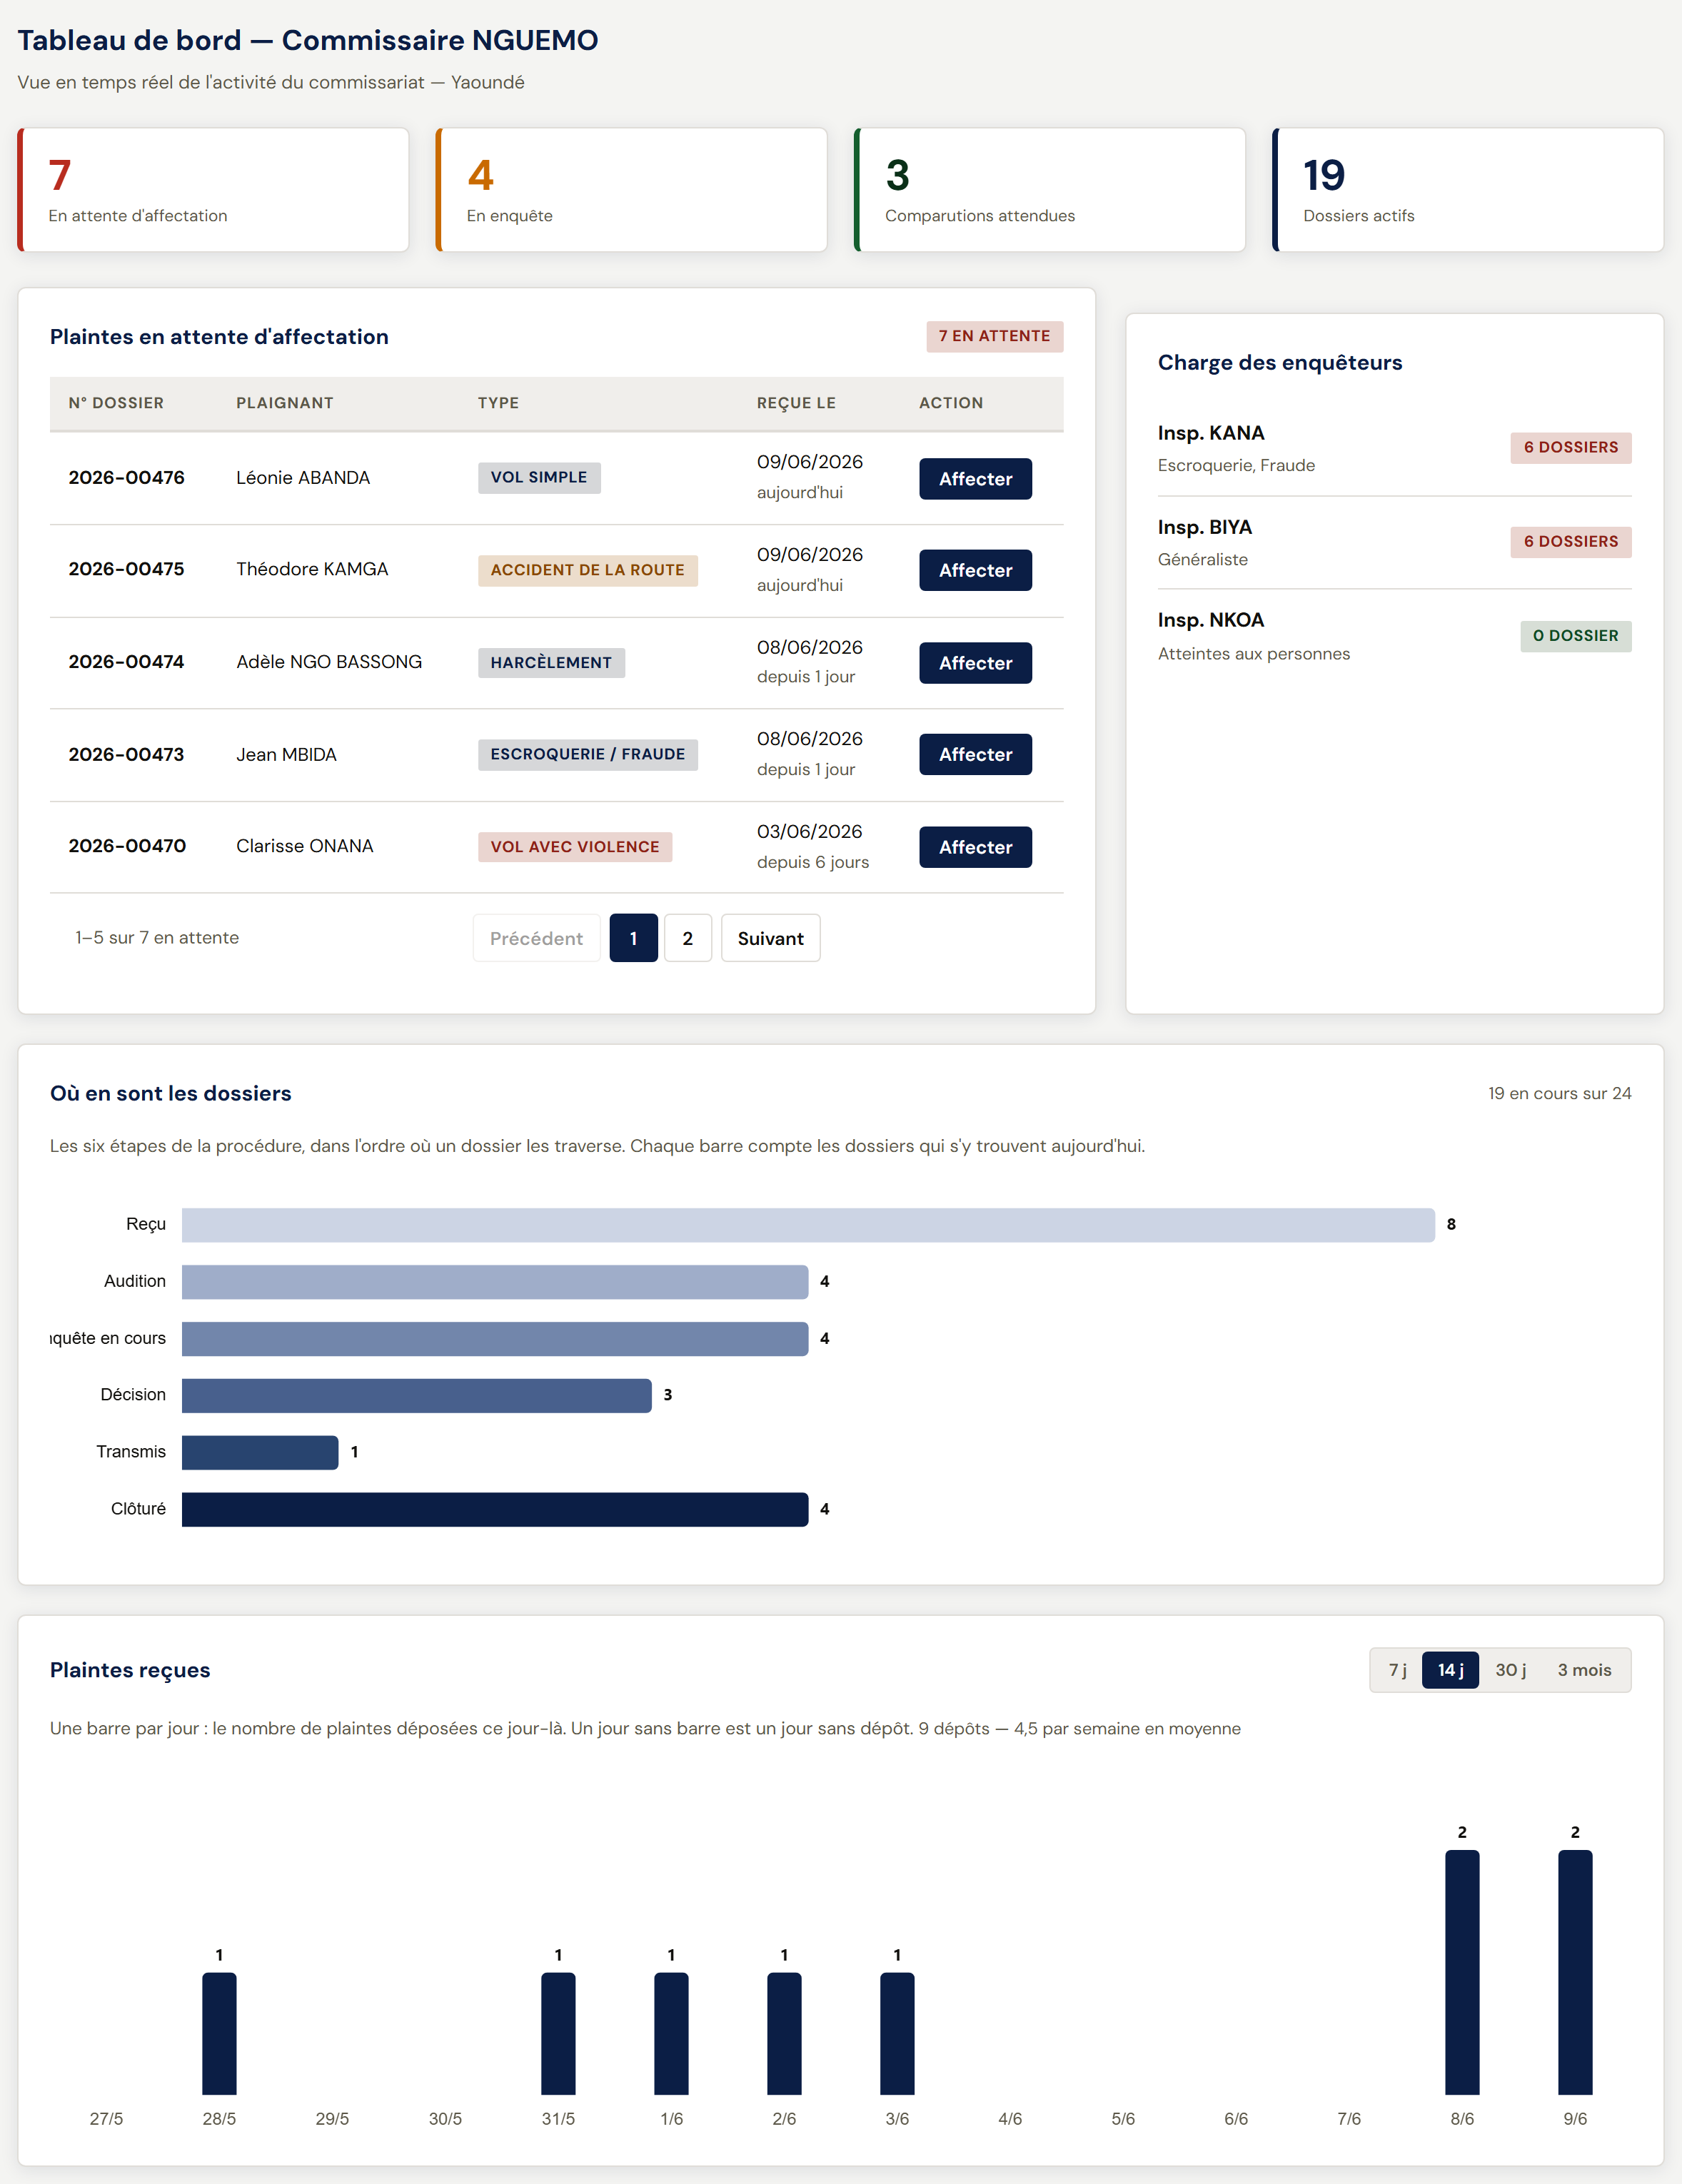
\includegraphics[width=0.58\textwidth]{images/dashboard.png}
    \caption{Tableau de bord du commissaire, vue générale}
    \label{fig:dashboard}
\end{figure}

Le tableau de bord réunit quatre indicateurs, à savoir les plaintes enregistrées, les dossiers achevés, le délai moyen de traitement et l'\textbf{avancement moyen des dossiers}, ainsi que la liste des dossiers récents et l'accès direct à la cotation. Le commissaire y trouve la vision d'ensemble de son unité que la procédure papier ne permettait pas sans dépouillement manuel du registre (BF8).

\subsection{Dépôt d'une plainte}

\begin{figure}[H]
    \centering
    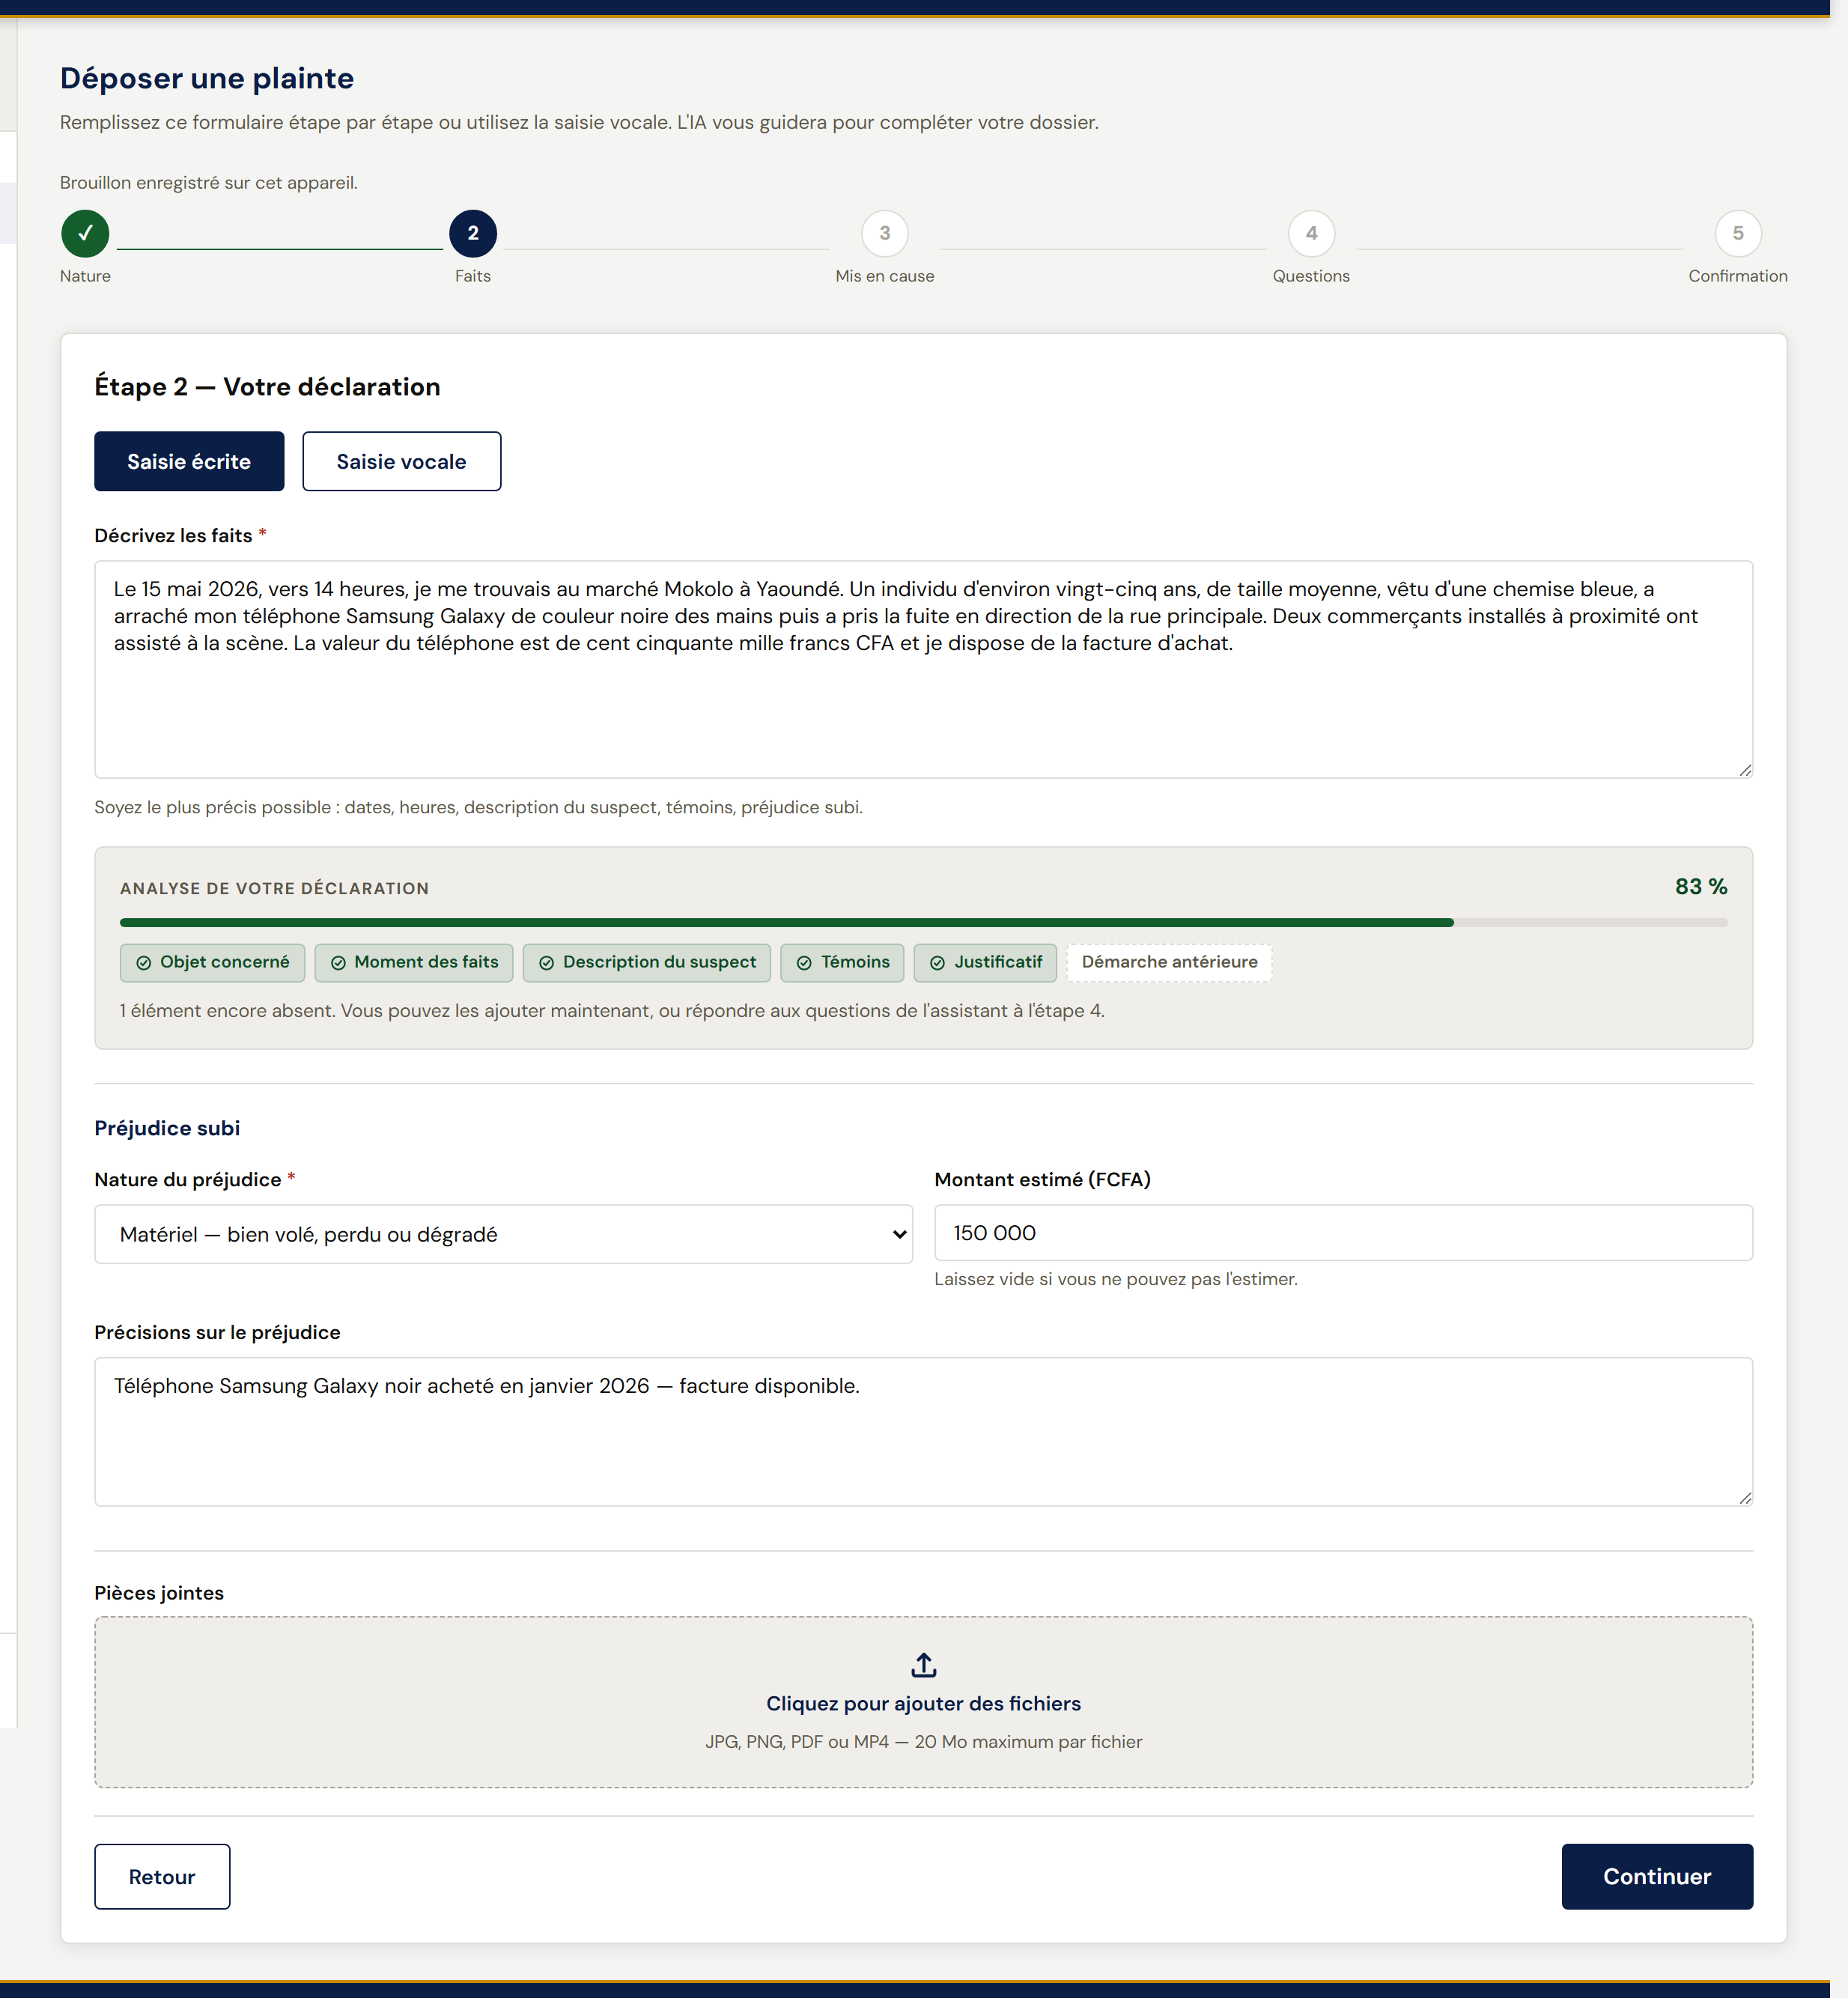
\includegraphics[width=0.58\textwidth]{images/modelisation.png}
    \caption{Parcours de dépôt guidé, formulaire en 5 étapes}
    \label{fig:soumission}
\end{figure}

Le parcours enchaîne le choix de la nature de l'infraction, la cascade géographique qui détermine le commissariat compétent, le récit libre des faits avec dictée vocale optionnelle, l'identité du mis en cause et les questions complémentaires. Une plainte peut ainsi être déposée intégralement en ligne, par un public non technicien et sans déplacement (BF1 et BF2).

\subsection{Instruction du dossier par l'enquêteur}

\begin{figure}[H]
    \centering
    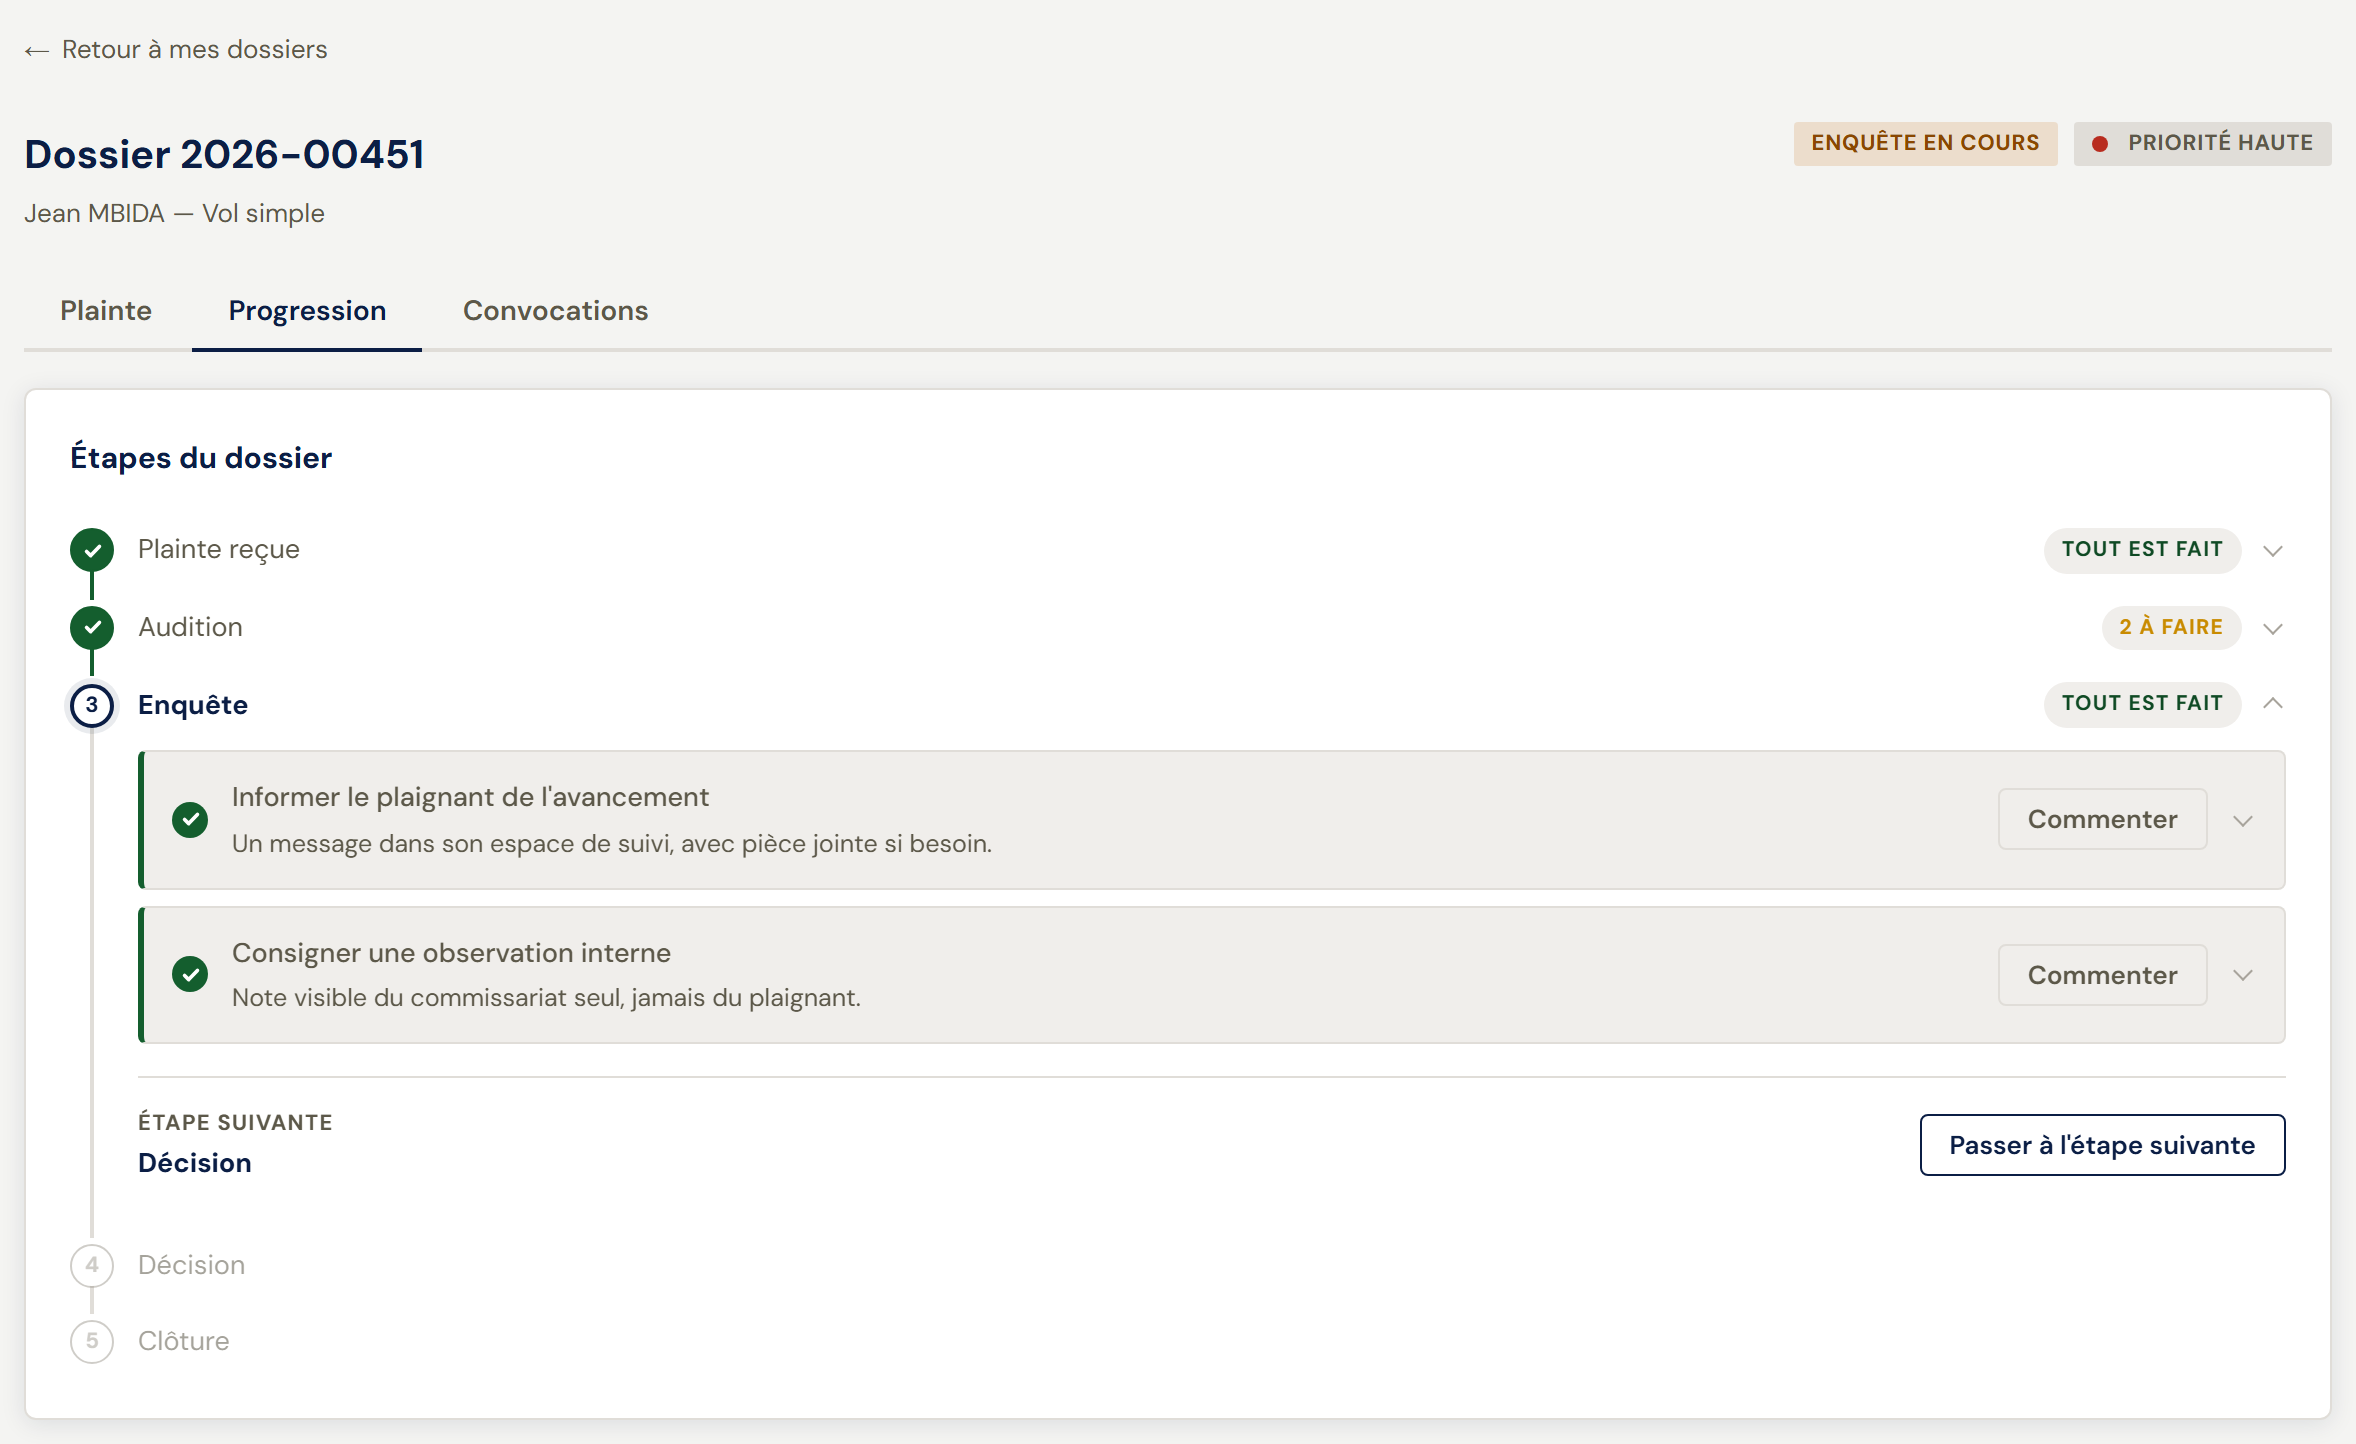
\includegraphics[width=0.58\textwidth]{images/configuration.png}
    \caption{Espace enquêteur, instruction d'un dossier et procès-verbal}
    \label{fig:configuration}
\end{figure}

L'enquêteur consulte le dossier coté, révise dans un éditeur le procès-verbal d'audition pré-rédigé, le valide, le signe et émet la convocation. Il part d'un document déjà structuré à partir de la déclaration du plaignant plutôt que d'une page blanche, sans que sa responsabilité en soit entamée : aucun procès-verbal n'est enregistré sans sa validation explicite (BF5).

\subsection{Gestion des dossiers cotés}

\begin{figure}[H]
    \centering
    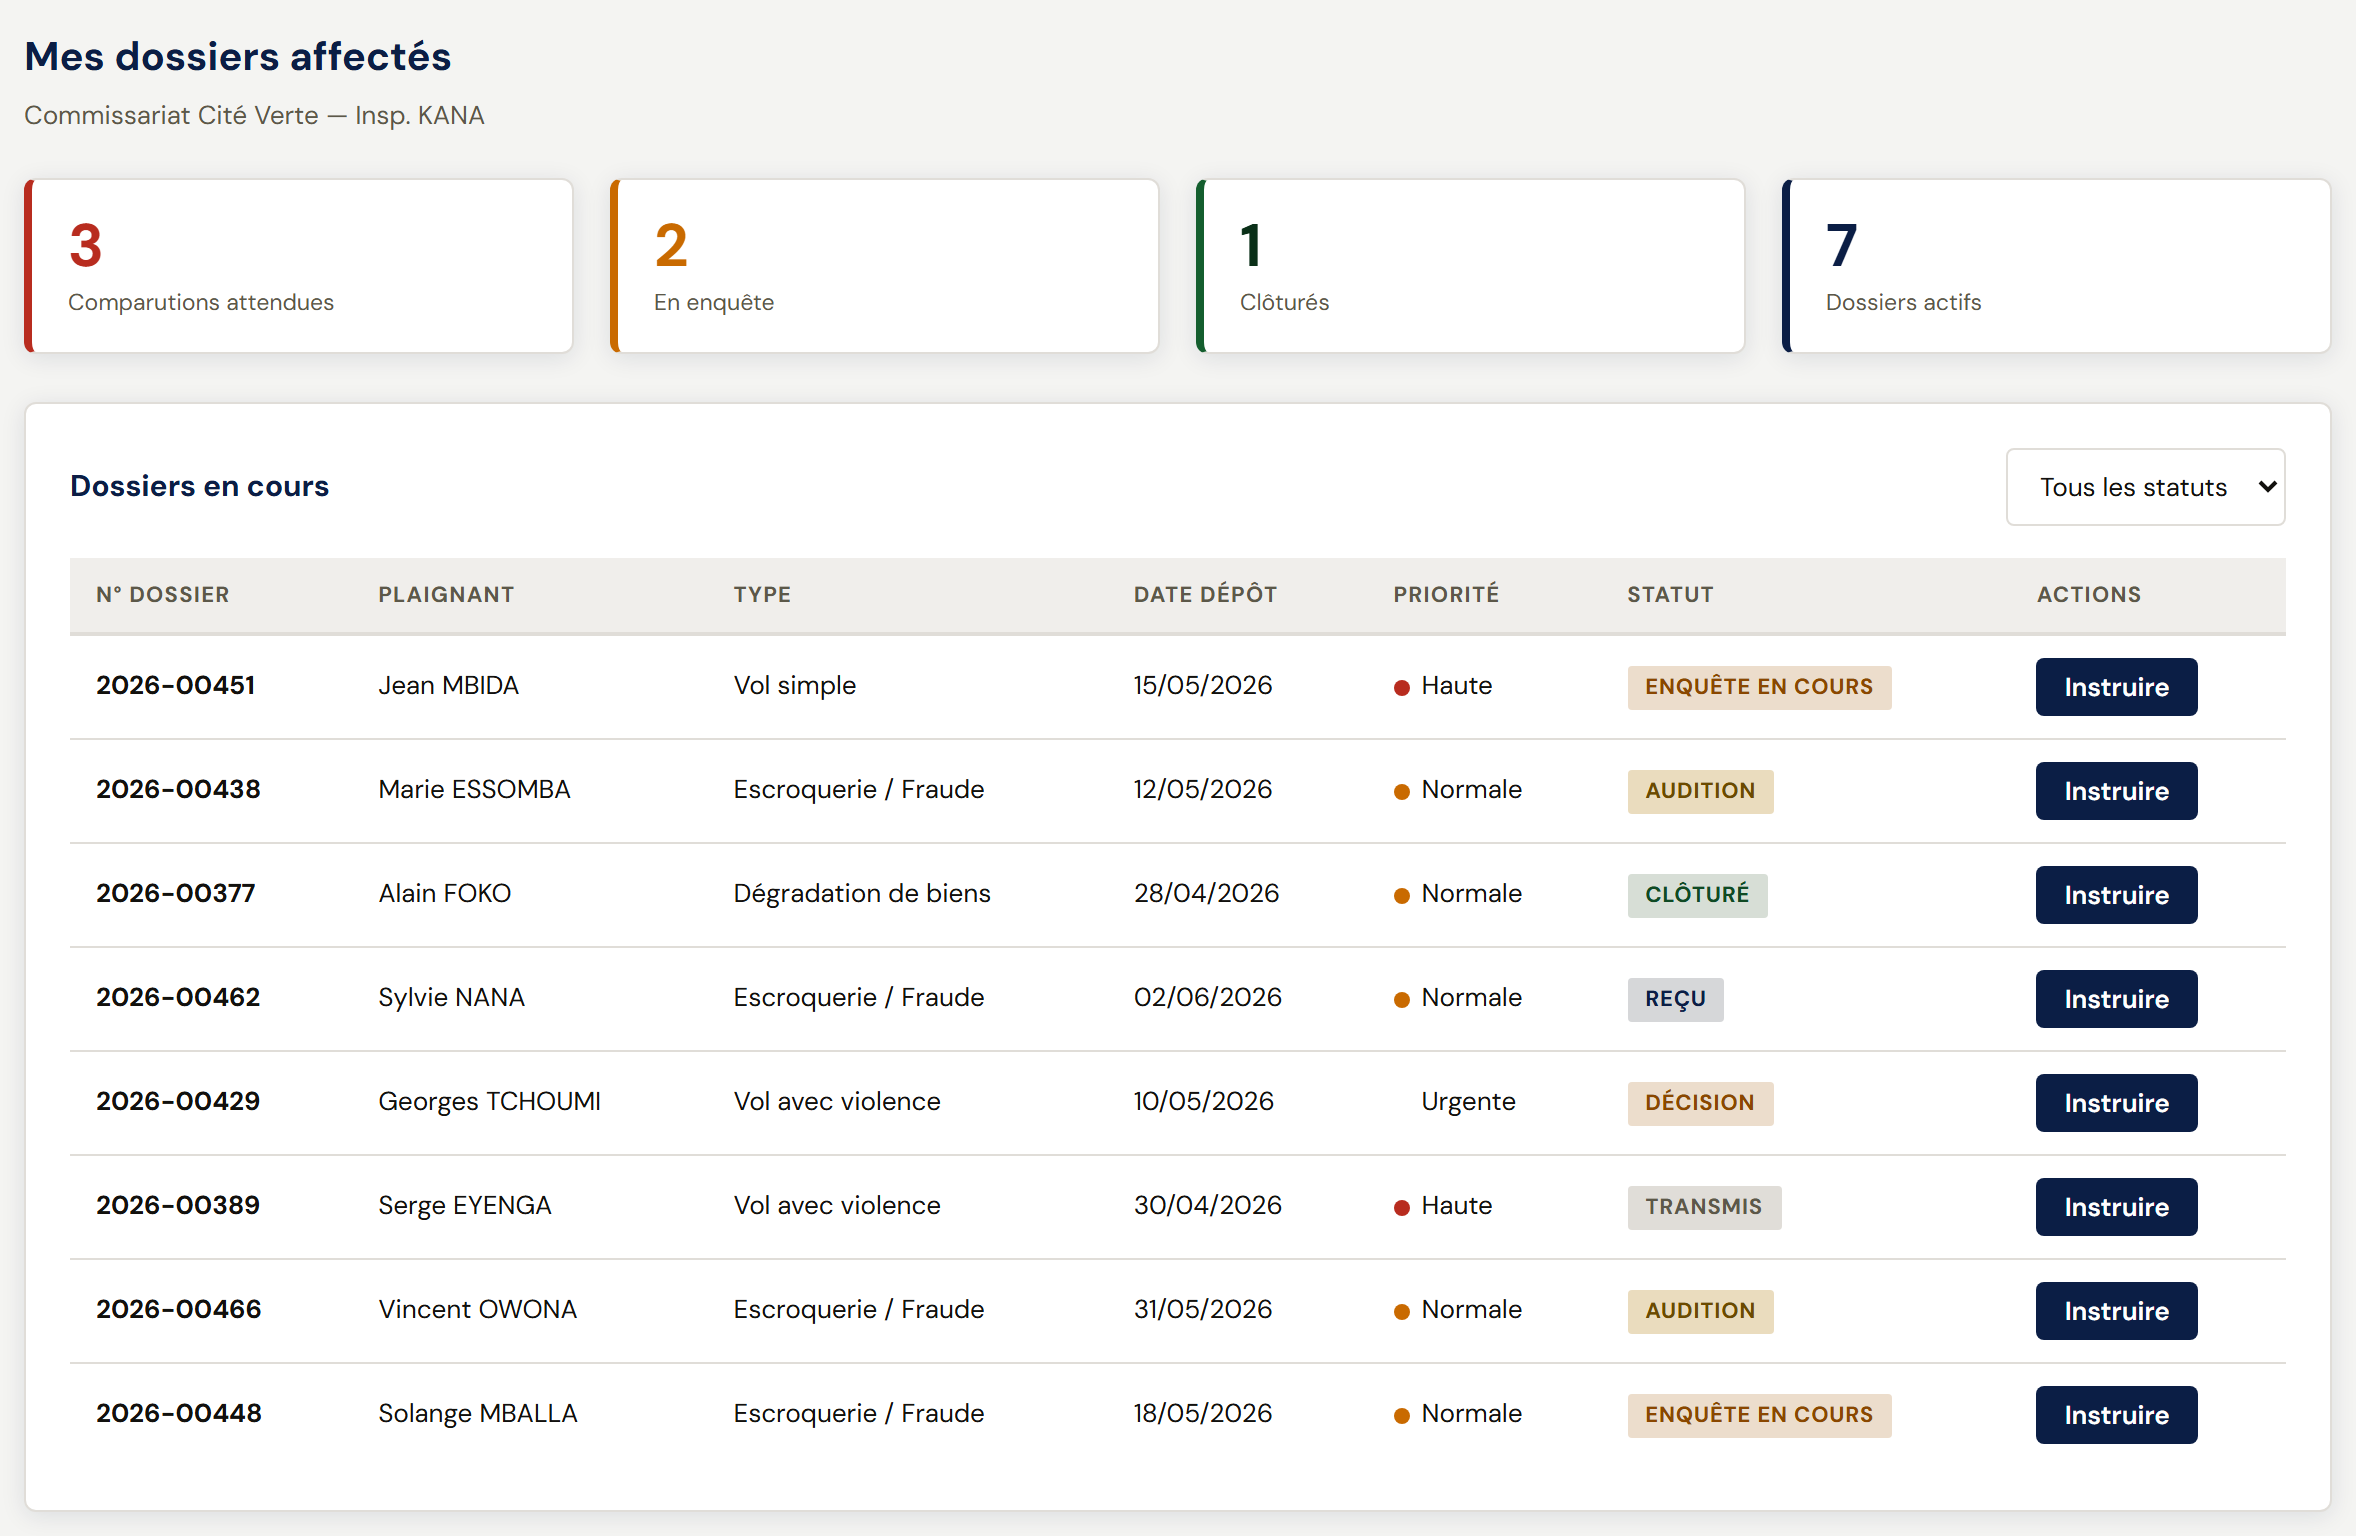
\includegraphics[width=0.58\textwidth]{images/task.png}
    \caption{Liste des dossiers cotés à l'enquêteur}
    \label{fig:taches}
\end{figure}

Chaque enquêteur dispose de son portefeuille de dossiers, classés par statut, filtrables par priorité et assortis d'actions rapides. Cette information était auparavant dispersée entre le registre et les chemises papier (BF4).

\subsection{Notifications}

\begin{figure}[H]
    \centering
    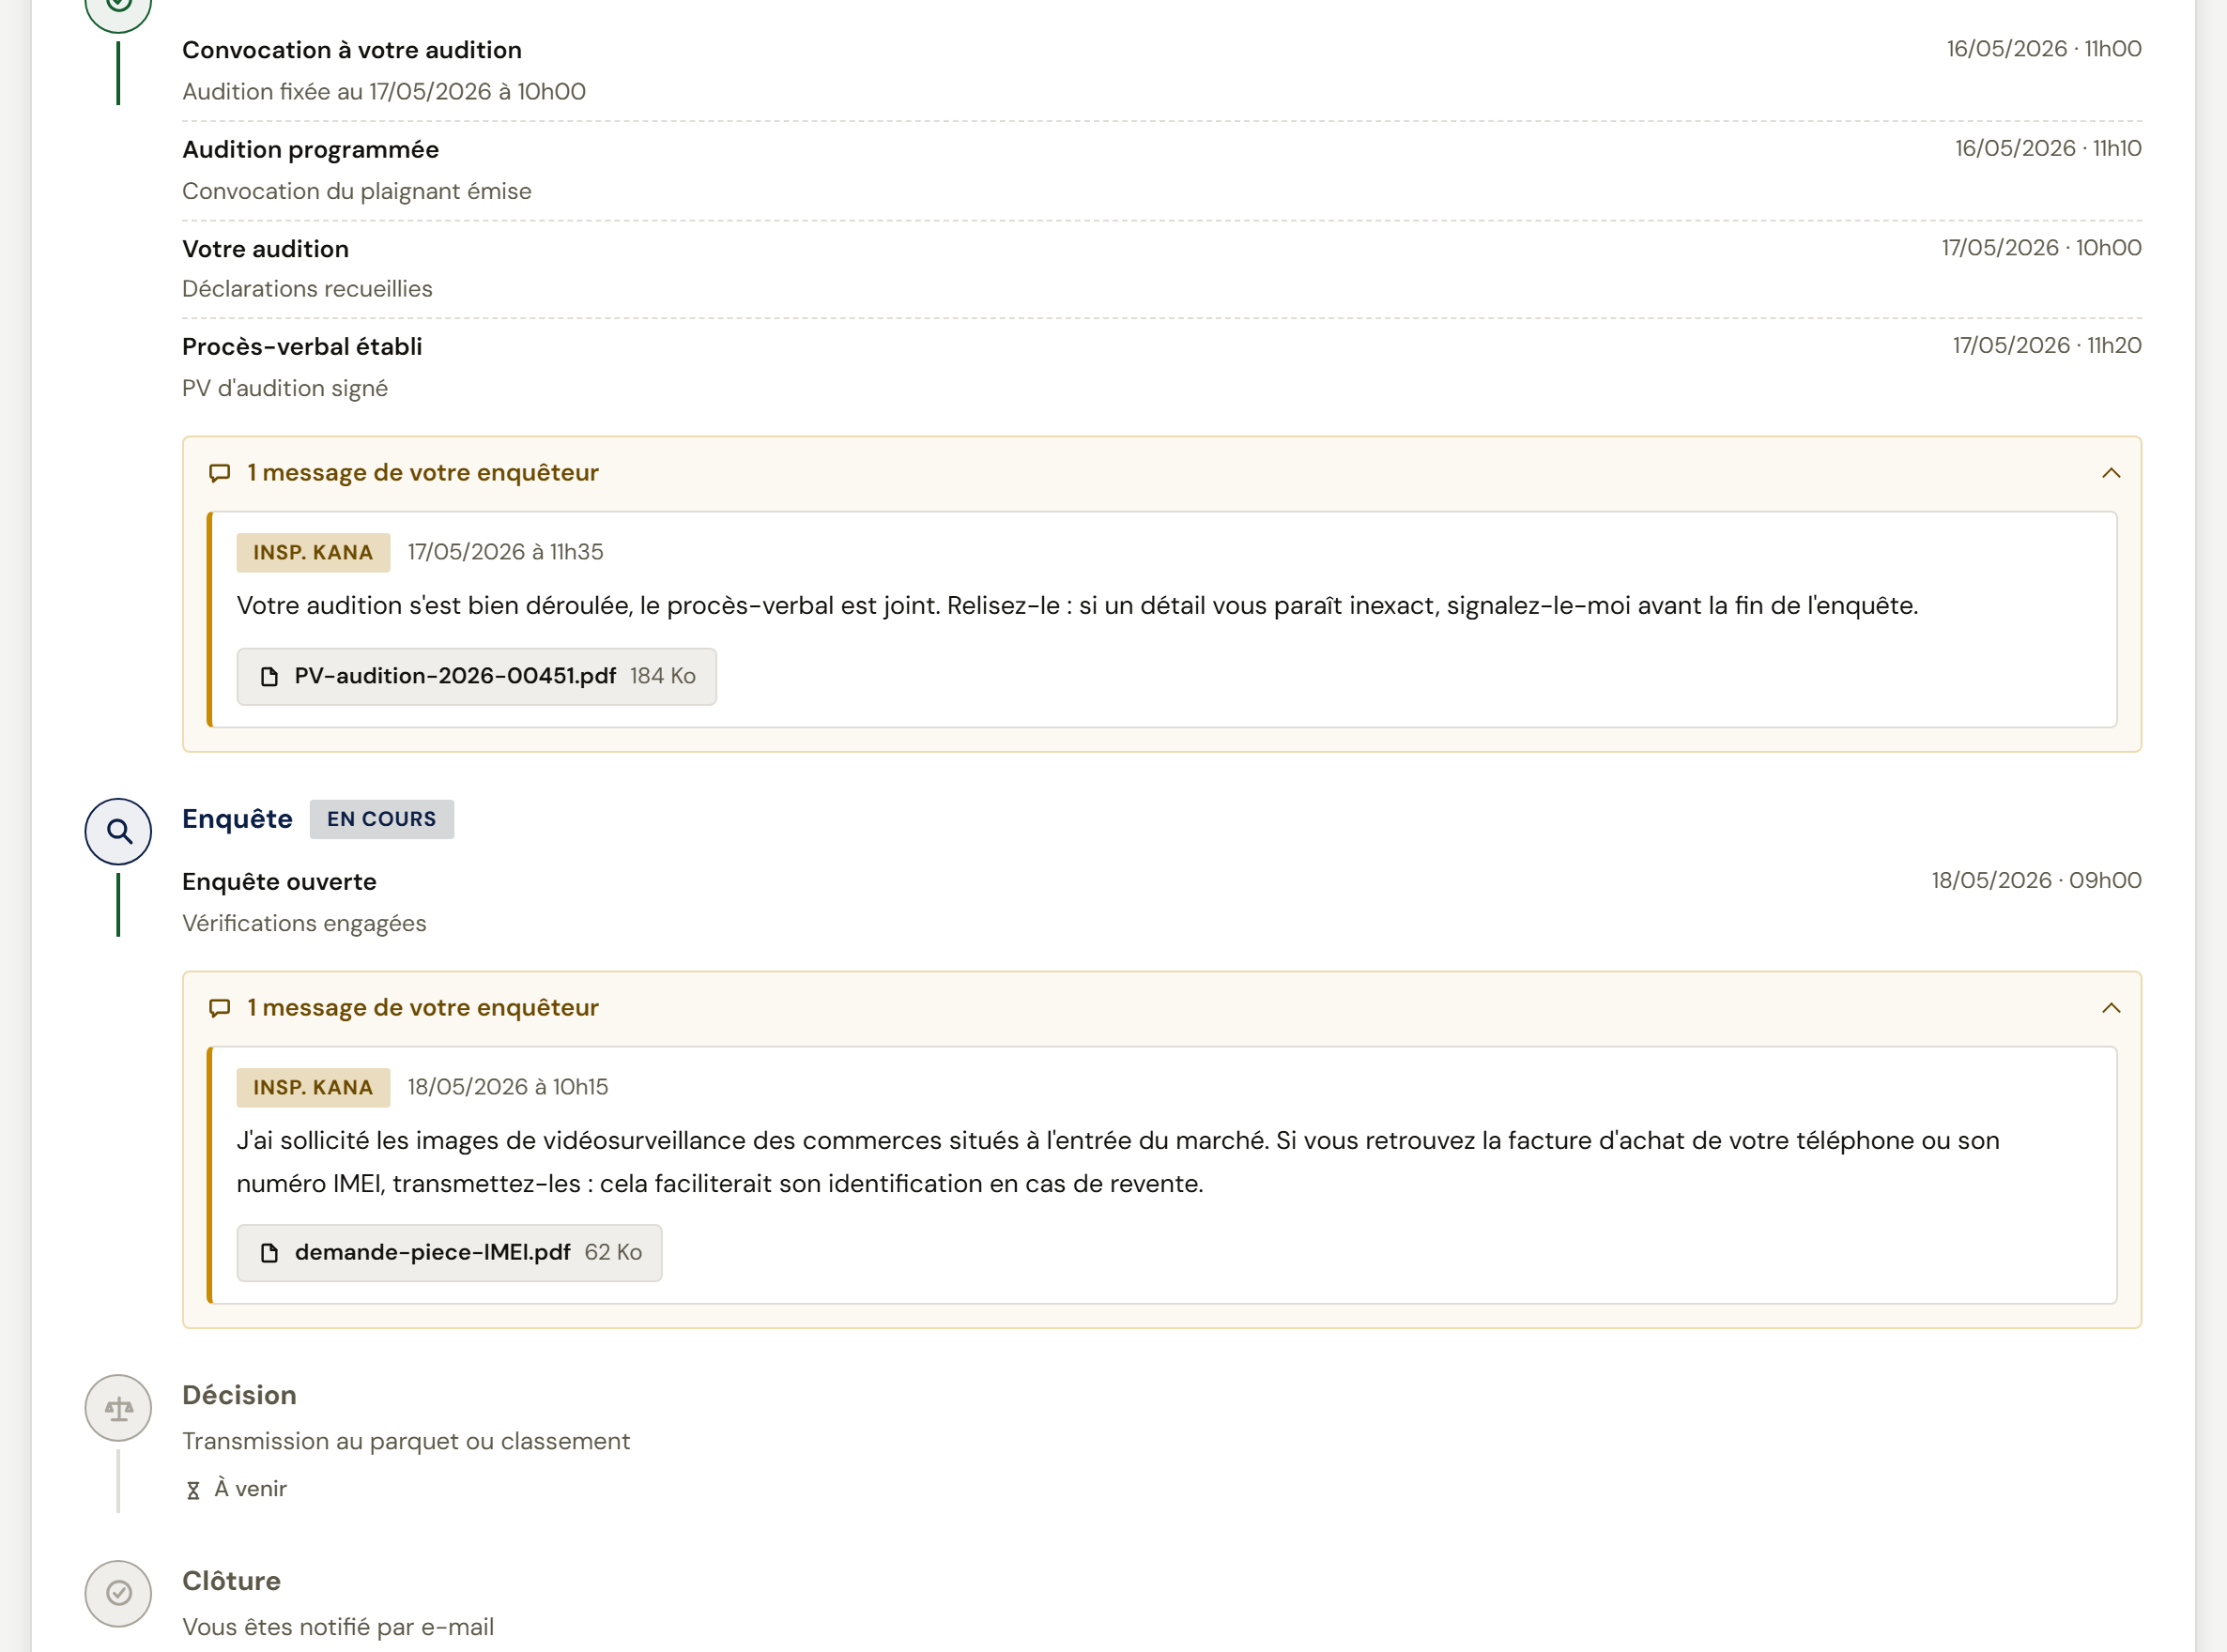
\includegraphics[width=0.58\textwidth]{images/notification.png}
    \caption{Centre de notifications}
    \label{fig:notifications}
\end{figure}

Changement de statut, convocation émise ou demande de pièce complémentaire : chaque notification porte un lien direct vers le dossier concerné. Le plaignant est informé de l'avancement de sa procédure sans se déplacer ni téléphoner au commissariat (BF6).

\subsection{Historique et traçabilité}

\begin{figure}[H]
    \centering
    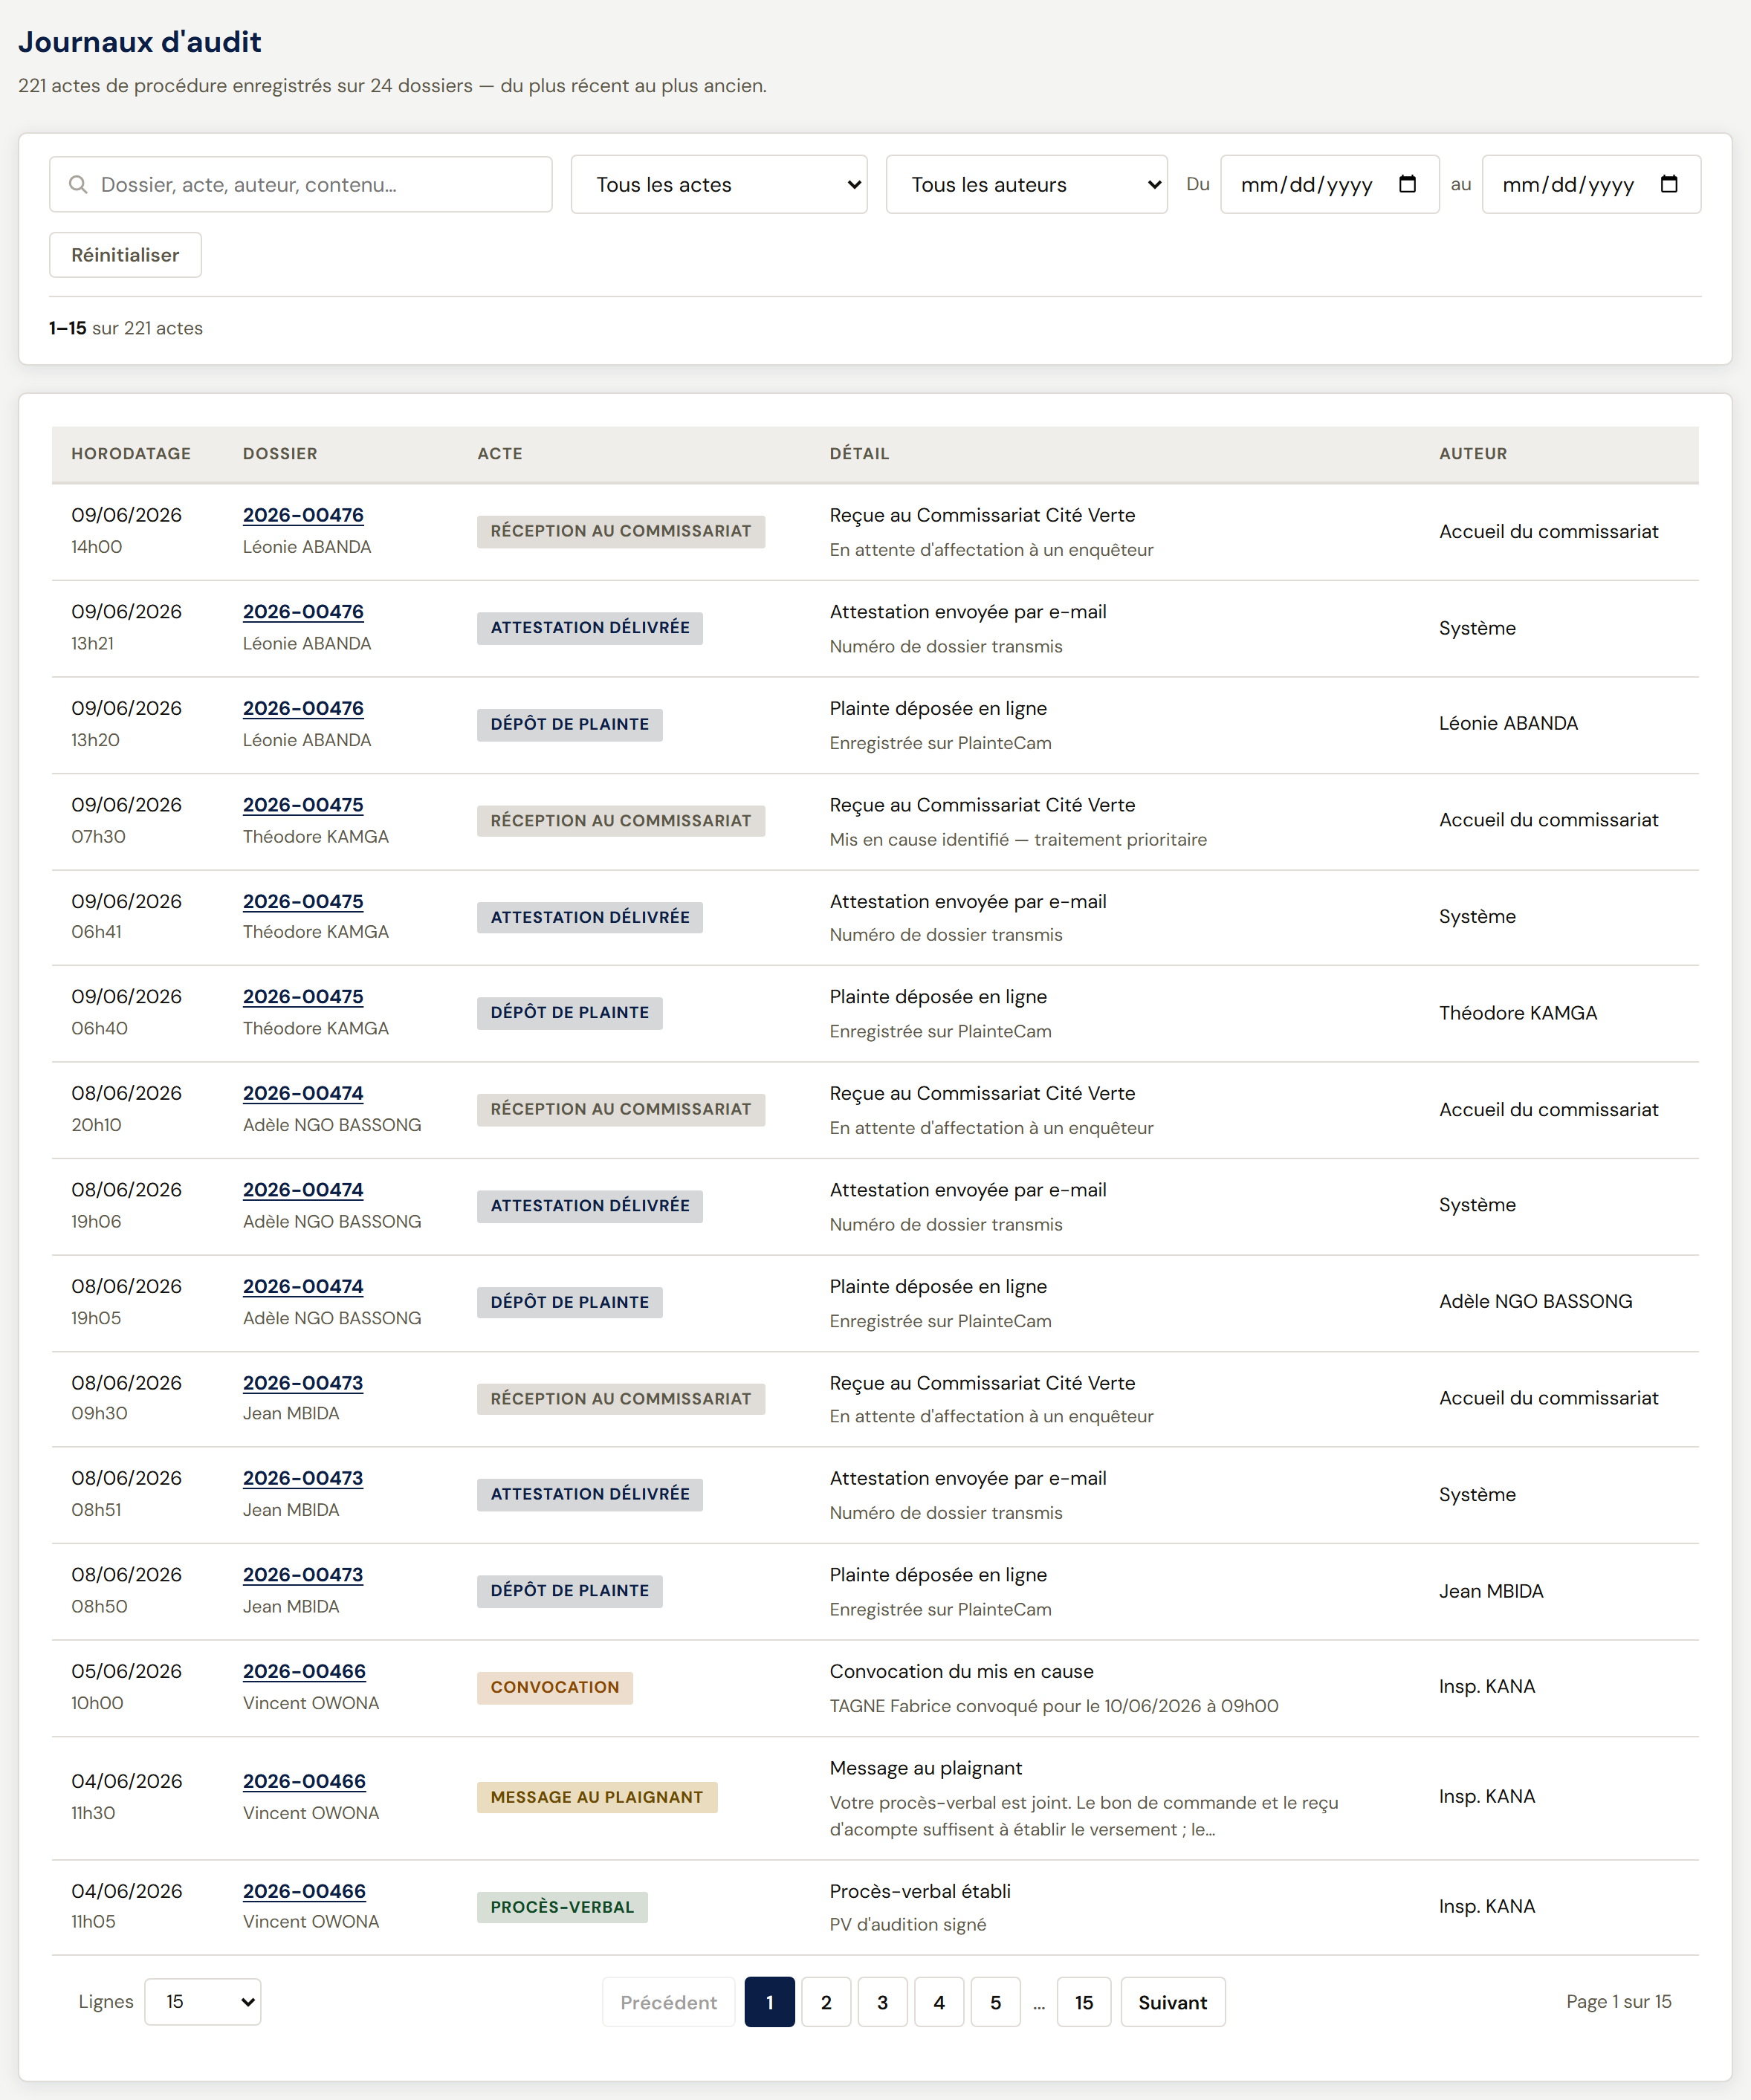
\includegraphics[width=0.58\textwidth]{images/historique.png}
    \caption{Journal d'audit, traçabilité de la procédure}
    \label{fig:historique}
\end{figure}

Chaque transition de statut, cotation, audition et validation de procès-verbal est horodatée et rattachée à son auteur. Ce journal constitue la contrepartie numérique du registre de main courante et fonde autant la conformité que le pilotage (BNF2).

\subsection{Statistiques et pilotage}

\begin{figure}[H]
    \centering
    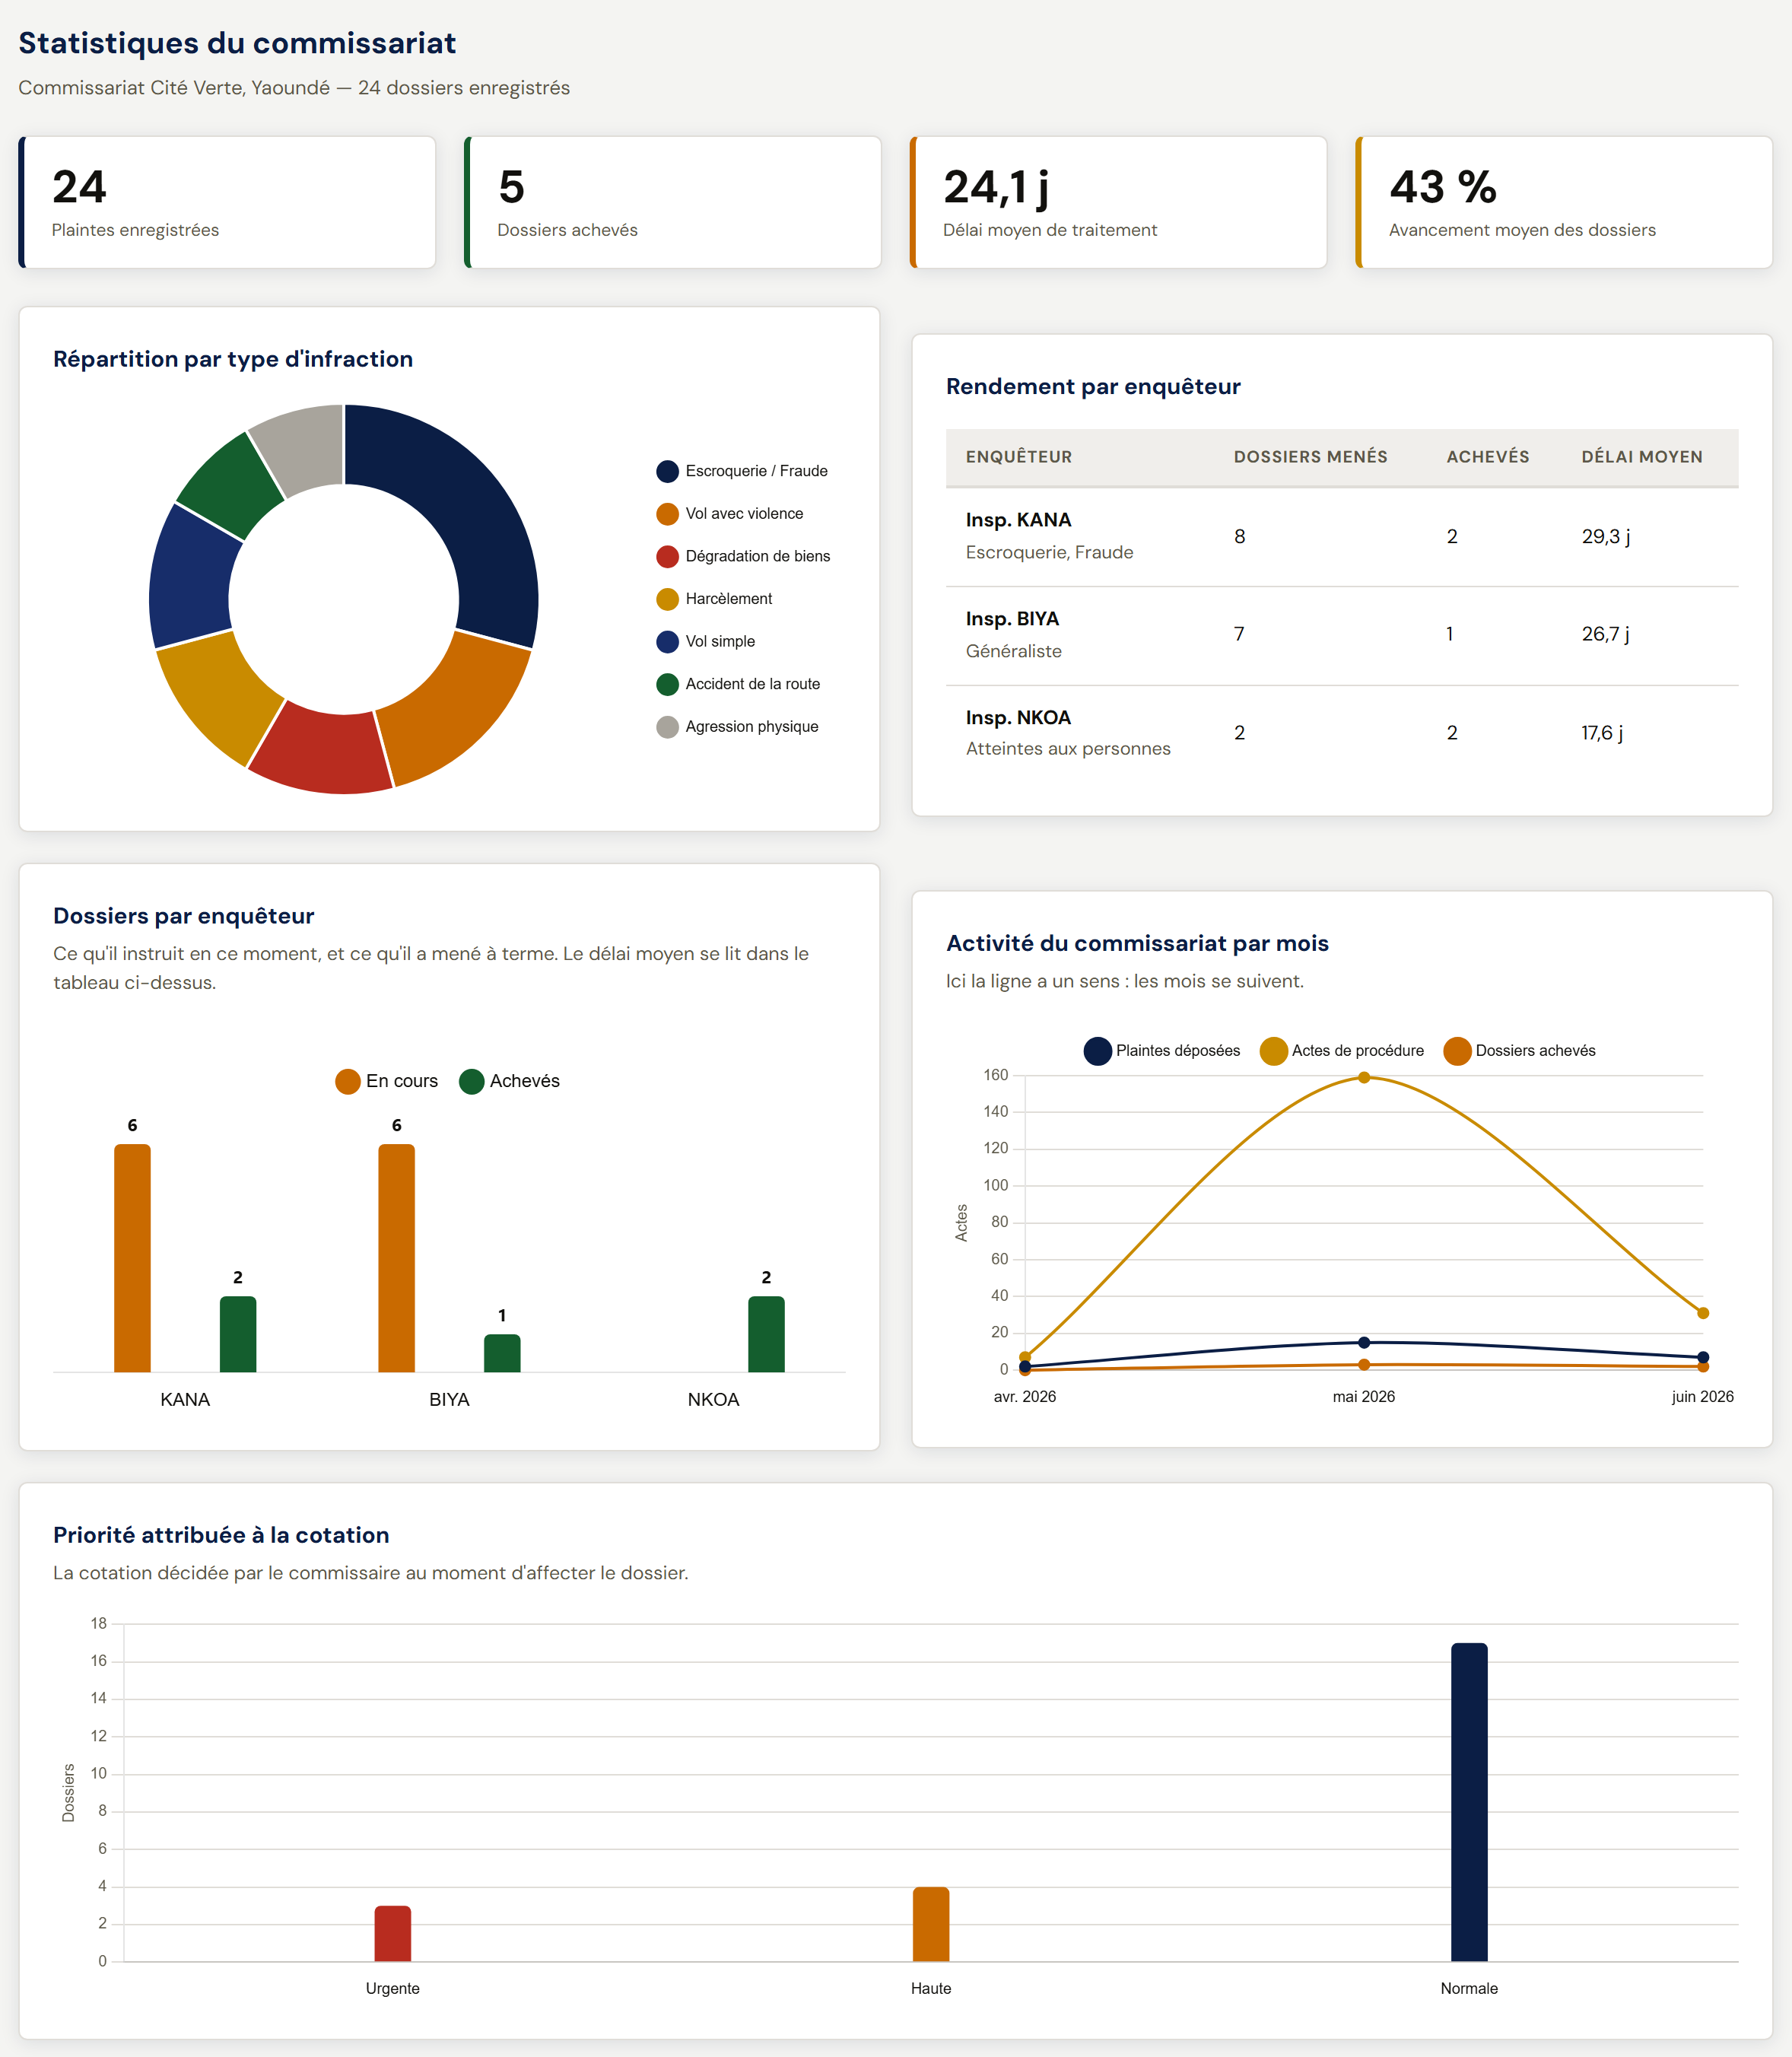
\includegraphics[width=0.58\textwidth]{images/avancee.png}
    \caption{Module de statistiques, répartitions et indicateurs}
    \label{fig:analyse}
\end{figure}

Répartition des plaintes par statut, par nature d'infraction et par priorité, charge par enquêteur : le commissaire dispose d'indicateurs objectifs pour répartir le travail et identifier les infractions dominantes sur son ressort.
